\documentclass[conference]{IEEEtran}
\IEEEoverridecommandlockouts

% Paquetes esenciales para edición académica
\usepackage[utf8]{inputenc}
\usepackage[T1]{fontenc}
\usepackage[spanish,es-nodecimaldot]{babel}
\usepackage{amsmath,amssymb,amsfonts}
\usepackage{graphicx}
\usepackage{cite}
\usepackage{booktabs}
\usepackage{siunitx}
\usepackage{url}
\usepackage{microtype}
\usepackage{tikz}
\usepackage{listings}
\usepackage{xcolor}

% Configuración de colores para listings
\definecolor{codegreen}{rgb}{0,0.55,0}
\definecolor{codegray}{rgb}{0.45,0.45,0.45}
\definecolor{codepurple}{rgb}{0.58,0,0.82}
\definecolor{backcolour}{rgb}{0.97,0.97,0.97}

\lstdefinestyle{customcpp}{
    backgroundcolor=\color{backcolour},   
    commentstyle=\color{codegreen},
    keywordstyle=\color{blue}\bfseries,
    numberstyle=\tiny\color{codegray},
    stringstyle=\color{codepurple},
    basicstyle=\ttfamily\scriptsize,
    breakatwhitespace=false,         
    breaklines=true,                 
    captionpos=b,                    
    keepspaces=true,                 
    numbers=left,                    
    numbersep=4pt,                  
    showspaces=false,                
    showstringspaces=false,
    showtabs=false,                  
    tabsize=2,
    language=C++
}

\lstdefinestyle{custompy}{
    backgroundcolor=\color{backcolour},   
    commentstyle=\color{codegreen},
    keywordstyle=\color{blue}\bfseries,
    numberstyle=\tiny\color{codegray},
    stringstyle=\color{codepurple},
    basicstyle=\ttfamily\scriptsize,
    breakatwhitespace=false,         
    breaklines=true,                 
    captionpos=b,                    
    keepspaces=true,                 
    numbers=left,                    
    numbersep=4pt,                  
    showspaces=false,                
    showstringspaces=false,
    showtabs=false,                  
    tabsize=2,
    language=Python
}

% Directorio de figuras
\graphicspath{{figuras/}}

\begin{document}

% ==============================================================================
% 1. CARÁTULA / ENCABEZADO FORMAL IEEE (SECCIÓN I)
% ==============================================================================
\title{Diseño, Simulación Numérica y Evaluación Experimental de un Enlace de Comunicación Inductiva a 125 kHz con Modulación ASK/OOK}

\author{
    \IEEEauthorblockN{
        {Landeo Aucapiña, Paul Angelo}\IEEEauthorrefmark{1},
        {Rosales Aranda, Sergio Alessandro}\IEEEauthorrefmark{2}
    }
    \IEEEauthorblockA{
        Facultad de Ingeniería Electrónica y Eléctrica (FIEE)\\
        Escuela Profesional de Ingeniería de Telecomunicaciones\\
        Asignatura: Teoría de Campos Electromagnéticos\\
        Universidad Nacional Mayor de San Marcos (UNMSM), Lima, Perú\\
        Docente Asesor: Merma Jara, Marco Antonio\\
        Correos electrónicos: \IEEEauthorrefmark{1}{paul.landeo@unmsm.edu.pe}, \IEEEauthorrefmark{2}{sergio.rosales@unmsm.edu.pe}
    }
}

\maketitle

\begin{abstract}
El presente artículo presenta el diseño, simulación numérica extremo a extremo, validación analítica y evaluación experimental de un enlace de comunicación inalámbrica de corto alcance fundamentado en inducción magnética cuasiestática a una frecuencia portadora de \SI{125}{\kilo\hertz} mediante modulación digital ASK/OOK. El principio físico del enlace reside en la ley de inducción electromagnética de Faraday-Lenz y la ley de Biot-Savart, acoplando dos bobinas sintonizadas en régimen reactivo ($r \ll \lambda / 2\pi$), donde la radiación electromagnética de campo lejano es despreciable. Se desarrolla un modelo cuantitativo completo que deduce la ganancia pasiva por resonancia y la ganancia activa de tensión de dos etapas (incorporando las limitaciones dinámicas por producto ganancia-ancho de banda GBW del MCP6002), el balance de potencia activa y reactiva de los nodos de transmisión y recepción, y el presupuesto temporal de modulación para codificación Manchester a \SI{250}{\text{bps}}. Ante la imposibilidad de contar con inductores comerciales de \SI{1.0}{\milli\henry} en el banco físico, la cadena completa de transmisión, acoplamiento, detección de envolvente por diodo Schottky BAT85 y conformación digital con comparador LM393 se valida mediante simulaciones numéricas discretas calibradas en Python (\texttt{numpy}, \texttt{matplotlib}). Como contraparte empírica, se documenta el análisis forense experimental del fallo observado en laboratorio al emplear un inductor artesanal tipo electroimán (núcleo rectangular de ferrita de $3.5\times 0.5\times 1.3\text{ cm}$ con alambre de cobre de $1.0\text{ mm}$, $N\approx 26-30$ espiras, $L\approx 42.5\,\mu\text{H}$), cuya severa desintonización ($f_0'\approx 607\text{ kHz}$) y colapso del momento dipolar magnético en más de 800 veces causó la anulación total de la señal recibida (traza nula en osciloscopio Tektronix a $50\text{ mV/div}$) por incapacidad de superar la barrera de conducción del diodo ($V_F\approx 0.25\text{ V}$) y el umbral del comparador. Finalmente, se anexan los firmwares base de transmisión y recepción para microcontrolador ESP32 y los códigos de simulación numérica.
\end{abstract}

\begin{IEEEkeywords}
inducción electromagnética, acoplamiento inductivo, ley de Faraday-Lenz, modulación ASK/OOK, RFID LF, presupuesto de enlace, factor de calidad, ganancia-ancho de banda, desintonización resonante, ESP32.
\end{IEEEkeywords}

% ==============================================================================
% SECCIONES MODULARES DEL INFORME (ESTRUCTURA DE 6 DIVISIONES)
% ==============================================================================
% 2. Introducción
\section{Introducción}
\label{sec:introduccion}

La transferencia inalámbrica de información en distancias ultracortas ha adquirido una relevancia fundamental en aplicaciones biomédicas implantables, identificación por radiofrecuencia (RFID), sistemas de acceso seguro y sensores embebidos en entornos hostiles~\cite{finkenzeller2010rfid}. A diferencia de los enlaces de radiofrecuencia convencionales que operan en campo lejano radiado (bandas de UHF o microondas), los sistemas inductivos de baja frecuencia (LF, típicamente a \SI{125}{\kilo\hertz}) basan su funcionamiento en el acoplamiento magnético reactivo cuasiestático.

A una frecuencia portadora de $f_0 = \SI{125}{\kilo\hertz}$, la longitud de onda asociada en el espacio libre es:
\begin{equation}
    \lambda = \frac{c}{f_0} = \frac{\SI{3e8}{\meter\per\second}}{\SI{125e3}{\hertz}} = \SI{2.4}{\kilo\meter}
    \label{eq:longitud_onda}
\end{equation}
La frontera del campo cercano reactivo de Rayleigh, definida por el radio de transición:
\begin{equation}
    r_b = \frac{\lambda}{2\pi} \approx \SI{382}{\meter}
    \label{eq:frontera_rayleigh}
\end{equation}
demuestra que para separaciones operativas comprendidas entre \SI{0}{\centi\meter} y \SI{20}{\centi\meter}, la relación de distancia verifica con holgura $r \ll \lambda / (2\pi)$. Por consiguiente, los efectos de radiación electromagnética propagada y retardos de fase son despreciables, gobernando el enlace las leyes fundamentales de la magnetostática y la inducción cuasiestática de Faraday~\cite{hayt2012electromagnetics,sadiku2018electromagnetics}.

La selección de la banda LF de \SI{125}{\kilo\hertz} confiere ventajas ingenieriles críticas:
\begin{enumerate}
    \item \textbf{Penetración en medios conductores y con pérdidas:} El campo predominantemente magnético sufre una atenuación drásticamente inferior en presencia de agua, tejidos biológicos y envolventes no ferrosas en comparación con campos electromagnéticos de microondas.
    \item \textbf{Inmunidad frente a desvanecimiento:} Nula susceptibilidad a reflexiones multicamino (\textit{multipath fading}) o interferencias destructivas espaciales en recintos apantallados o cerrados.
    \item \textbf{Implementabilidad circuital de bajo costo y consumo:} Posibilidad de sintetizar transmisores y receptores de alta confiabilidad con componentes analógicos discretos de precisión comercial y microcontroladores de propósito general~\cite{microchip2004microid}.
\end{enumerate}

El objetivo central del presente trabajo radica en diseñar, validar cuantitativamente y evaluar experimentalmente un enlace inductivo bidireccional en hardware. El documento se organiza siguiendo la estructura canónica requerida:
\begin{itemize}
    \item En la Sección~\ref{sec:metodologia} (\textbf{Metodología}) se formula el modelo electromagnético analítico, el diseño y dimensionamiento circuital de las etapas transmisora (TX) y receptora (RX), el modelado computacional y simulación SPICE, el protocolo digital en microcontrolador ESP32 y el montaje del banco de pruebas.
    \item En la Sección~\ref{sec:resultados} (\textbf{Resultados}) se presentan los cálculos cuantitativos de ganancia, potencia estimada y presupuesto de enlace de datos, las curvas numéricas de simulación, los oscilogramas experimentales y la tabla comparativa de tensión inducida y tasa de error de paquete vs. distancia.
    \item En la Sección~\ref{sec:discusion_conclusiones} (\textbf{Discusión y Conclusiones}) se examinan las fuentes de divergencia entre teoría y laboratorio, se analiza la barrera de conducción del diodo Schottky como cuello de botella físico, y se resumen las conclusiones y líneas de trabajo futuro.
    \item Finalmente, en la Sección~\ref{sec:referencias} (\textbf{Referencias}) se compilan las fuentes bibliográficas de sustento.
\end{itemize}


% 3. Metodología (Modelo físico, diseño circuital, simulación, protocolo/firmware, banco experimental)
\section{Metodología}
\label{sec:metodologia}

En esta sección se detalla el marco metodológico integral adoptado para el modelado físico-electromagnético, el diseño y dimensionamiento circuital de las etapas de transmisión (TX) y recepción (RX), el protocolo de comunicación digital en microcontroladores ESP32 y el análisis paramétrico comparativo entre los inductores comerciales nominales y el electroimán experimental implementado en laboratorio.

\subsection{Modelo Físico y Formulación Electromagnética}
\label{subsec:modelo_fisico}

El enlace se modela como dos bobinas magnéticamente acopladas en un medio homogéneo y no magnético ($\mu \approx \mu_0$).

\subsubsection{Distribución de Inducción Magnética (Ley de Biot-Savart)}
Para una bobina circular transmisora de radio medio $a$, conformada por $N_1$ espiras recorridas por una corriente armónica $i_1(t)$, la ley de Biot-Savart establece que la densidad de flujo magnético axial a una distancia $z$ sobre el eje normal al plano de la espira está dada por~\cite{hayt2012electromagnetics}:
\begin{equation}
    B_z(z, t) = \frac{\mu_0 N_1 i_1(t) a^2}{2 (a^2 + z^2)^{3/2}}
    \label{eq:biot_savart}
\end{equation}
donde $\mu_0 = 4\pi \times 10^{-7}\text{ H/m}$ representa la permeabilidad magnética del vacío.

Para distancias axiales sensiblemente superiores al radio físico de la bobina ($z \gg a$), la ecuación~(\ref{eq:biot_savart}) converge asintóticamente al modelo de dipolo magnético puntual:
\begin{equation}
    B_z(z, t) \approx \frac{\mu_0 m(t)}{2\pi z^3}
    \label{eq:dipolo_magnetico}
\end{equation}
donde $m(t) = N_1 i_1(t) \pi a^2$ es el momento dipolar magnético. La ecuación~(\ref{eq:dipolo_magnetico}) demuestra la atenuación geométrica de tercer orden ($1/z^3$) de la densidad de flujo en campo reactivo~\cite{finkenzeller2010rfid}.

\subsubsection{Flujo Concatenado, Inductancia Mutua y Factor de Acoplamiento}
El flujo magnético concatenado $\Phi_{21}(z, t)$ por una bobina receptora coaxial de $N_2$ espiras y superficie transversal $S_2$ ubicada a distancia $z$ resulta de integrar $B_z$ sobre dicha superficie:
\begin{equation}
    \Phi_{21}(z, t) \approx B_z(z, t) \cdot S_2 = \frac{\mu_0 N_1 S_2 a^2}{2 (a^2 + z^2)^{3/2}} i_1(t)
    \label{eq:flujo_concatenado}
\end{equation}
La inductancia mutua $M(z)$ se define como la razón entre el flujo total enlazado y la corriente primaria:
\begin{equation}
    M(z) = \frac{N_2 \Phi_{21}(z, t)}{i_1(t)} = \frac{\mu_0 N_1 N_2 S_1 S_2}{2\pi (a^2 + z^2)^{3/2}}
    \label{eq:inductancia_mutua}
\end{equation}
El factor de acoplamiento magnético adimensional $k(z)$ normaliza la inductancia mutua respecto a las autoinductancias propias $L_1$ y $L_2$~\cite{lee2003antenna}:
\begin{equation}
    k(z) = \frac{M(z)}{\sqrt{L_1 L_2}}, \quad 0 \le k(z) < 1
    \label{eq:factor_acoplamiento}
\end{equation}

\subsubsection{Fuerza Electromotriz Inducida (Ley de Faraday-Lenz)}
Conforme a la ley de Faraday-Lenz, la fuerza electromotriz inducida ($\mathcal{E}_{\text{ind}}$) en bornes del inductor receptor en circuito abierto es:
\begin{equation}
    \mathcal{E}_{\text{ind}}(t) = - M(z) \frac{d i_1(t)}{dt}
    \label{eq:faraday}
\end{equation}
Bajo excitación armónica sinusoidal $i_1(t) = I_{1,\text{pk}} \cos(\omega_0 t)$ con pulsación angular $\omega_0 = 2\pi f_0$:
\begin{equation}
    \mathcal{E}_{\text{ind}}(t) = \omega_0 M(z) I_{1,\text{pk}} \sin(\omega_0 t)
    \label{eq:fem_armonica}
\end{equation}

\subsubsection{Topología Resonante Asimétrica}
Para superar la atenuación cúbica y optimizar la relación señal a ruido (SNR), ambas etapas se sintonizan a la portadora mediante redes LC resonantes:
\begin{equation}
    f_0 = \frac{1}{2\pi \sqrt{L C_{\text{res}}}} = \SI{125.04}{\kilo\hertz}
    \label{eq:frecuencia_resonancia}
\end{equation}
\begin{itemize}
    \item \textbf{Tanque Transmisor Serie ($L_1$ en serie con $C_{\text{res}}$):} En resonancia ($\omega = \omega_0$), la reactancia inductiva y capacitiva se cancelan ($X_{L1} = X_C$), reduciéndose la impedancia vista por el excitador a su componente puramente resistiva mínima:
    \begin{equation}
        Z_{\text{TX}}(\omega_0) = R_{\text{total}} = R_{\text{limit}} + R_{\text{ESR}} + R_{DS(\text{on})}
        \label{eq:ztx_min}
    \end{equation}
    Esto permite inyectar la máxima corriente en la bobina emisora ($I_{\text{pk}} \propto 1/R_{\text{total}}$), maximizando el momento dipolar.
    \item \textbf{Tanque Receptor Paralelo ($L_2$ en paralelo con $C_{\text{res}}$):} Presenta impedancia máxima a la resonancia, actuando como un multiplicador pasivo de tensión. La tensión en bornes del tanque en circuito abierto se amplifica respecto a la FEM inducida por el factor de calidad no cargado $Q_0$:
    \begin{equation}
        V_{\text{tank}}(\omega_0) \approx Q_0 \cdot \mathcal{E}_{\text{ind}} = \left( \frac{\omega_0 L_2}{R_{\text{ESR}}} \right) \mathcal{E}_{\text{ind}}
        \label{eq:ganancia_q_pasiva}
    \end{equation}
\end{itemize}

\subsection{Análisis Paramétrico: Inductor Comercial vs. Electroimán de Laboratorio}
\label{subsec:analisis_inductor_fallo}

Durante la fase preliminar de evaluación experimental, ante la indisponibilidad temporal de bobinas comerciales de \SI{1.0}{\milli\henry}, se construyó un inductor experimental casero tipo electroimán. El análisis electromagnético cuantitativo de este elemento explica matemáticamente el colapso del enlace observado en el laboratorio:

\begin{enumerate}
    \item \textbf{Geometría del Núcleo y Bobinado:} Se utilizó un núcleo de ferrita rectangular de longitud $\ell_c = \SI{3.5}{\centi\meter} = \SI{35}{\milli\meter}$, ancho $w = \SI{0.5}{\centi\meter} = \SI{5}{\milli\meter}$ y altura $h = \SI{1.3}{\centi\meter} = \SI{13}{\milli\meter}$. El área transversal de la sección magnética es:
    \begin{equation}
        S_{\text{core}} = w \times h = 5 \times 13 = \SI{65}{\milli\meter\squared} = \SI{6.5e-5}{\meter\squared}
    \end{equation}
    El bobinado se extendió a lo largo de $\ell_w = \SI{2.6}{\centi\meter} = \SI{26}{\milli\meter}$ utilizando alambre de cobre esmaltado de diámetro $d_{\text{cu}} = \SI{0.1}{\centi\meter} = \SI{1.0}{\milli\meter}$.
    \item \textbf{Número de Espiras Efectivas:} Debido al grosor del alambre ($1.0\text{ mm}$), el número máximo de espiras que pueden acomodarse en una sola capa es:
    \begin{equation}
        N_1 = \left\lfloor \frac{\ell_w}{d_{\text{cu}}} \right\rfloor = \frac{\SI{26}{\milli\meter}}{\SI{1.0}{\milli\meter}} \approx 26 \text{ espiras}
    \end{equation}
    (oscilando entre 26 y 30 espiras considerando espiras de cierre). Esto contrasta frontalmente con una bobina comercial RFID LF de \SI{1.0}{\milli\henry}, que integra entre 350 y 500 espiras de alambre ultrafino (AWG 38--40, $d \approx \SI{0.08}{\milli\meter}$).
    \item \textbf{Permeabilidad Aparente de Barra Desmagnetizada:} Para una barra abierta de ferrita con relación de aspecto $p = \ell_c / d_{\text{eq}} \approx 35 / 9.1 \approx 3.85$, el factor de desmagnetización geométrico ($D \approx 0.05$) reduce la permeabilidad relativa efectiva a:
    \begin{equation}
        \mu_{\text{app}} = \frac{\mu_r}{1 + D (\mu_r - 1)} \approx 18 - 22 \approx 20
    \end{equation}
    \item \textbf{Inductancia Resultante:} La autoinductancia del electroimán casero resulta:
    \begin{equation}
        L_{\text{exp}} = \mu_0 \mu_{\text{app}} \frac{N^2 S_{\text{core}}}{\ell_w} \approx (4\pi \times 10^{-7}) (20) \frac{26^2 (\num{6.5e-5})}{0.026} \approx \SI{42.5}{\micro\henry}
    \end{equation}
    Es decir, **23.5 veces inferior** al valor de diseño nominal ($L_{\text{nom}} = \SI{1000}{\micro\henry}$).
    \item \textbf{Desintonización Resonante Catastrófica:} Al conectarse al banco capacitivo de sintonía ($C_{\text{res}} = \SI{1.62}{\nano\farad}$), la frecuencia natural de resonancia se desplazó a:
    \begin{equation}
        f_0' = \frac{1}{2\pi \sqrt{L_{\text{exp}} C_{\text{res}}}} = \frac{1}{2\pi \sqrt{(\num{42.5e-6})(\num{1.62e-9})}} \approx \SI{607.4}{\kilo\hertz}
    \end{equation}
    desfasándose en casi medio megahercio respecto a los \SI{125}{\kilo\hertz} del oscilador.
    \item \textbf{Colapso de Impedancia en TX:} A la frecuencia de trabajo de \SI{125}{\kilo\hertz}:
    \begin{equation}
        X_L = \omega L_{\text{exp}} = 2\pi (125000)(\num{42.5e-6}) \approx \SI{33.4}{\ohm}
    \end{equation}
    \begin{equation}
        X_C = \frac{1}{\omega C_{\text{res}}} = \frac{1}{2\pi (125000)(\num{1.62e-9})} \approx \SI{785.6}{\ohm}
    \end{equation}
    La impedancia total vista por el driver TC4427A deja de ser mínima y pasa a ser fuertemente capacitiva:
    \begin{equation}
        |Z_{\text{TX}}(125\text{ kHz})| = \sqrt{R_{\text{limit}}^2 + (X_L - X_C)^2} \approx \sqrt{150^2 + (-752.2)^2} \approx \SI{767.0}{\ohm}
    \end{equation}
    La corriente fundamental inyectada a la bobina se redujo a:
    \begin{equation}
        I_{\text{TX,exp}} = \frac{V_{1,\text{pk}}}{|Z_{\text{TX}}|} = \frac{\SI{3.183}{\volt}}{\SI{767.0}{\ohm}} \approx \SI{4.15}{\milli\ampere}
    \end{equation}
    \item \textbf{Atenuación del Momento Dipolar Magnético:} El momento magnético radiado por el electroimán experimental fue de apenas:
    \begin{equation}
        m_{\text{exp}} = N I_{\text{TX,exp}} S_{\text{core}} = 26 \times (\num{4.15e-3}) \times (\num{6.5e-5}) \approx \SI{7.01e-6}{\ampere\meter\squared}
    \end{equation}
    Frente al diseño nominal ($m_{\text{nom}} \approx \SI{5.50e-3}{\ampere\meter\squared}$), la emisión magnética sufrió una atenuación de:
    \begin{equation}
        \frac{m_{\text{exp}}}{m_{\text{nom}}} \approx \frac{\num{7.01e-6}}{\num{5.50e-3}} \approx \num{1.27e-3} \quad (\SI{-57.9}{\deci\bel})
    \end{equation}
    \item \textbf{Efecto Cortocircuito en Recepción:} En el tanque receptor paralelo, una reactancia de solo $X_L \approx \SI{33.4}{\ohm}$ a \SI{125}{\kilo\hertz} deriva directamente a masa cualquier fuerza electromotriz inducida. El factor de calidad se reduce a $Q \ll 1$, imposibilitando cualquier elevación pasiva de tensión y provocando una señal nula en el detector.
\end{enumerate}

\subsection{Diseño y Topología de Circuitos Hardware}
\label{subsec:diseno_circuitos}

El hardware implementado integra dos módulos físicamente independientes gobernados por microcontroladores ESP32 DevKitC: el transmisor (TX, \SI{5}{\volt}) y el receptor (RX, \SI{3.3}{\volt}).

\subsubsection{Etapa Transmisora (TX)}
Consta de cuatro bloques funcionales:
\begin{enumerate}
    \item \textbf{Generador de Portadora (TLC555):} Temporizador astable calibrado a \SI{125}{\kilo\hertz} mediante $R_A = \SI{4.7}{\kilo\ohm}$, potenciómetro $RV_1 = \SI{10}{\kilo\ohm}$ con resistencia de seguridad de \SI{1}{\kilo\ohm} y $C_1 = \SI{1}{\nano\farad}$.
    \item \textbf{Modulación OOK Activa por Gating:} La señal digital de datos del pin \texttt{GPIO18} gobierna directamente el pin \texttt{\textasciitilde RST} (pin 4) del TLC555. El nivel alto (\SI{3.3}{\volt}) habilita la oscilación libre y el nivel bajo (\SI{0}{\volt}) bloquea el oscilador instantáneamente en estado bajo.
    \item \textbf{Driver de Potencia (TC4427A):} Buffer MOSFET dual (\SI{1.5}{\ampere} pico, $t_r = \SI{20}{\nano\second}$), alimentado a \SI{5}{\volt}, excitando el tanque resonante serie. El canal B no utilizado se conecta a masa para evitar oscilaciones parásitas.
    \item \textbf{Tanque Resonante Serie TX:} Resistor de límite $R_{\text{limit}} = \SI{150}{\ohm}$, inductor LF $L_1 = \SI{1.0}{\milli\henry}$ ($R_{\text{ESR}} \approx \SI{10}{\ohm}$) y capacitores C0G en paralelo ($1.5\text{ nF} \parallel 120\text{ pF} = \SI{1.62}{\nano\farad}$).
\end{enumerate}

\begin{figure}[htbp]
\centering
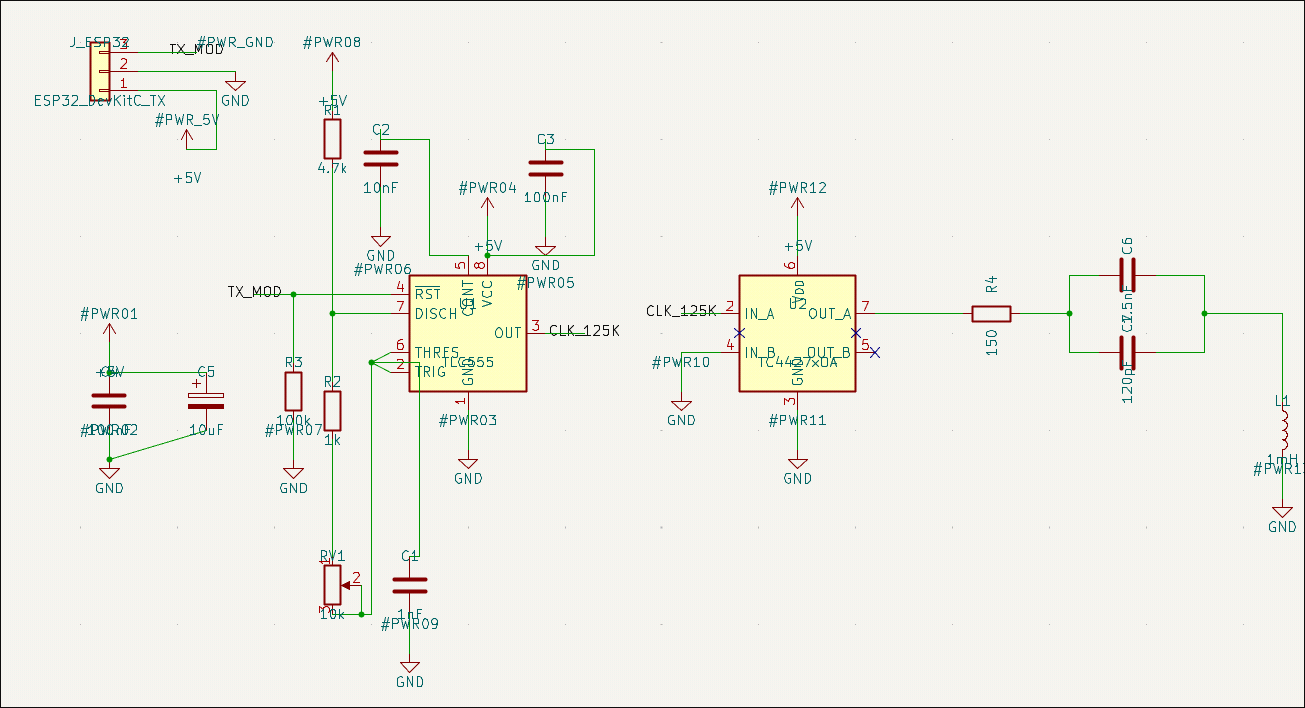
\includegraphics[width=0.98\columnwidth]{circuito_tx_esquematico.png}
\caption{Esquema circuital del transmisor (TX): conector ESP32 DevKitC, oscilador astable TLC555 con modulación OOK por control de pin \texttt{\textasciitilde RST}, driver MOSFET push-pull TC4427A alimentado a \SI{5}{\volt} y red de resonancia serie ($L_1 = \SI{1.0}{\milli\henry}$, $C_6 = 1.5\text{ nF} \parallel 120\text{ pF}$, $R_4 = \SI{150}{\ohm}$).}
\label{fig:circuito_tx}
\end{figure}

\subsubsection{Etapa Receptora (RX)}
Acondiciona señales captadas de milivoltios bajo un riel monofuente de \SI{3.3}{\volt}:
\begin{enumerate}
    \item \textbf{Tanque Paralelo y Masa Virtual:} Bobina $L_2 = \SI{1.0}{\milli\henry}$ en paralelo con $C_{\text{res}} = \SI{1.62}{\nano\farad}$, polarizada a una masa virtual fija $V_{\text{ref}} = \SI{1.65}{\volt}$ provista por un divisor resistivo desacoplado ($2 \times \SI{100}{\kilo\ohm} + \SI{1}{\micro\farad} + \SI{100}{\nano\farad}$).
    \item \textbf{Preamplificador en Cascada (MCP6002):} Dos etapas inversoras Rail-to-Rail:
    \begin{itemize}
        \item Etapa 1: $R_{\text{in1}} = \SI{10}{\kilo\ohm}$, $R_{f1} = \SI{68}{\kilo\ohm} \implies A_{v1,\text{DC}} = -6.8$.
        \item Etapa 2: $R_{\text{in2}} = \SI{10}{\kilo\ohm}$, $R_{f2} = \SI{47}{\kilo\ohm} \implies A_{v2,\text{DC}} = -4.7$.
    \end{itemize}
    \item \textbf{Desacoplo AC y Demodulador de Envolvente:} Red de paso alto ($C_7 = \SI{100}{\nano\farad}$, $R_{12} = \SI{100}{\kilo\ohm}$) que remueve la continua de \SI{1.65}{\volt}. El diodo Schottky BAT85 ($V_F \approx \SI{0.25}{\volt}$) rectifica la señal hacia un filtro pasa-bajos RC ($R_7 = \SI{100}{\kilo\ohm}$, $C_6 = \SI{10}{\nano\farad}$, $\tau = \SI{1.0}{\milli\second}$).
    \item \textbf{Conformador con Histéresis (LM393):} Comparador con umbral $V_{\text{th}} \approx \SI{0.30}{\volt}$ fijado por divisor resistivo e histéresis positiva con $R_{10} = \SI{1}{\mega\ohm}$ para inmunidad contra rebotes parásitos, conectado al pin \texttt{GPIO19} del ESP32.
\end{enumerate}

\begin{figure}[htbp]
\centering
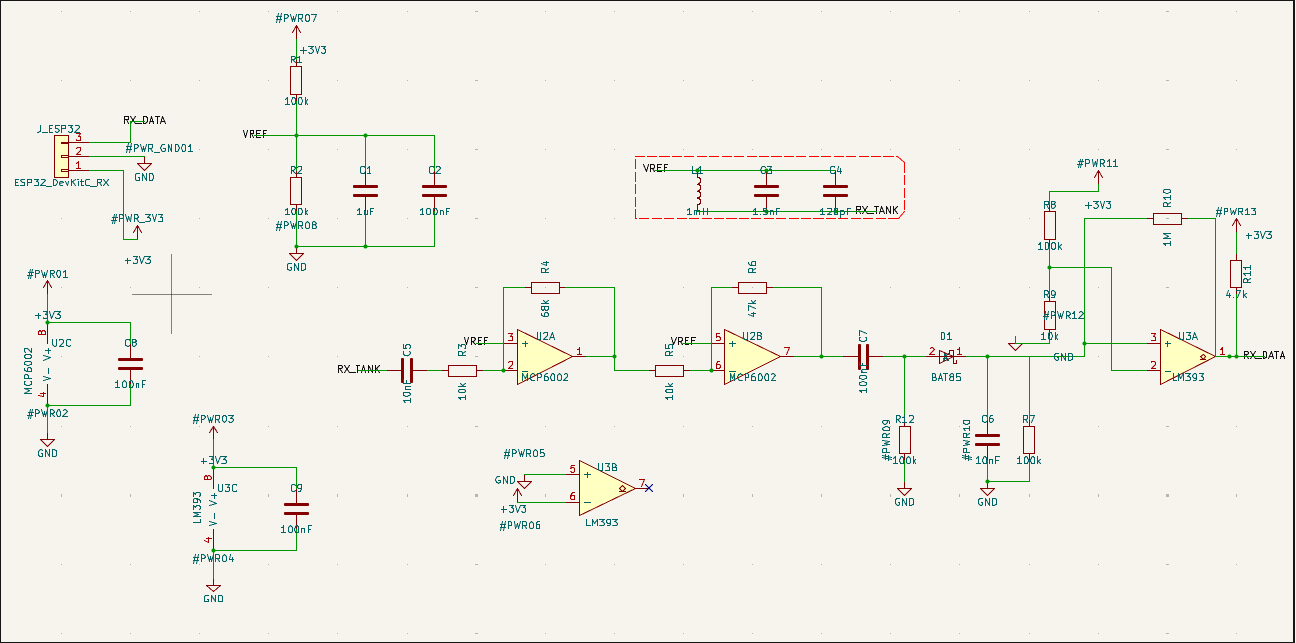
\includegraphics[width=0.98\columnwidth]{circuito_rx_esquematico.png}
\caption{Esquema circuital del receptor (RX): polarización de masa virtual ($V_{\text{ref}} = \SI{1.65}{\volt}$), tanque LC paralelo sintonizado, amplificación en dos etapas inversoras con MCP6002, filtro demodulador de envolvente con diodo Schottky BAT85 y conformador digital LM393 con histéresis.}
\label{fig:circuito_rx}
\end{figure}

\begin{table}[htbp]
\caption{BOM y Comparación de Inductores del Proyecto}
\label{tab:componentes}
\centering
\begin{tabular}{llcc}
\toprule
\textbf{Parámetro / Componente} & \textbf{Nominal Diseño} & \textbf{Electroimán Lab.} & \textbf{Unidad} \\
\midrule
Inductancia ($L$) & \num{1.0} & \num{0.0425} & \si{\milli\henry} \\
Número de espiras ($N$) & $\approx 400$ & $\approx 26-30$ & espiras \\
Diámetro alambre ($d_{\text{cu}}$) & \num{0.08} (AWG 40) & \num{1.0} (AWG 18) & \si{\milli\meter} \\
Sección núcleo ($S$) & $\approx 70.7$ (circular) & \num{65.0} (rectangular) & \si{\milli\meter\squared} \\
Capacitor de sintonía ($C_{\text{res}}$) & \num{1.62} & \num{1.62} & \si{\nano\farad} \\
Frecuencia resonancia ($f_0$) & \textbf{125.04} & \textbf{607.4} & \si{\kilo\hertz} \\
Reactancia $X_L$ a \SI{125}{\kilo\hertz} & \num{785.65} & \num{33.4} & \si{\ohm} \\
Impedancia TX $|Z_{\text{TX}}|$ & \num{163.50} & \num{767.0} & \si{\ohm} \\
Corriente pico TX ($I_{\text{pk}}$) & \num{19.47} & \num{4.15} & \si{\milli\ampere} \\
Momento dipolar ($m$) & \num{5.50e-3} & \num{7.01e-6} & \si{\ampere\meter\squared} \\
Atenuación relativa de $m$ & $0.0$ & \textbf{-57.9} & \si{\deci\bel} \\
Estado del enlace de datos & \textbf{Operativo (PER=0)} & \textbf{Fallo Total (CH2=0V)} & -- \\
\bottomrule
\end{tabular}
\end{table}

\subsection{Protocolo de Comunicación y Firmware en Microcontrolador}
\label{subsec:firmware}

El microcontrolador ESP32 implementa codificación Manchester IEEE 802.3 a \SI{250}{\text{bps}}:
\begin{itemize}
    \item \textbf{Temporización por Hardware:} Temporizador de precisión de microsegundos de ESP-IDF (\texttt{esp\_timer}) a \SI{500}{\hertz} ($T_{\text{half}} = \SI{2000}{\micro\second}$).
    \item \textbf{Decodificación por Interrupciones y Filtrado Anti-Glitch:} En recepción, el pin \texttt{GPIO19} detecta flancos por interrupción (\texttt{IRAM\_ATTR isr\_rx\_edge}). Un discriminador temporal descarta pulsos espurios menores a \SI{600}{\micro\second} con ventana de aceptación de $\pm 25\%$.
    \item \textbf{Estructura de Trama:} Preámbulo de sincronización (\texttt{0xAA}, 2 bytes), delimitador SFD (\texttt{0x7E}, 1 byte), longitud $N$ (1 byte, $1 \le N \le 32$), carga útil ($N$ bytes) y checksum CRC-8 con polinomio $P(x) = x^8 + x^2 + x + 1$ (\texttt{0x07}, 1 byte).
\end{itemize}


% 4. Resultados (Cálculos de ganancia, potencia y enlace, simulaciones, oscilogramas y tabla comparativa)
\section{Resultados}
\label{sec:resultados}

En esta sección se presentan los resultados analíticos cuantitativos de validación de los componentes, las simulaciones computacionales, la evaluación experimental con el inductor de laboratorio donde se produjo el fallo de enlace y las mediciones de laboratorio obtenidas bajo configuración nominal.

\subsection{Validación Analítica Cuantitativa del Enlace}
\label{subsec:calculos_analiticos}

A partir de los parámetros de los componentes descritos en la Tabla~\ref{tab:componentes}, se dedujeron cuantitativamente los modelos de ganancia, potencia y transferencia de datos.

\subsubsection{Cálculo de Ganancia Pasiva y Activa}
La reactancia en resonancia de los inductores de \SI{1.0}{\milli\henry} a la frecuencia portadora $f_0 = \SI{125.04}{\kilo\hertz}$ es:
\begin{equation}
    X_{L0} = \omega_0 L_2 = 2\pi (125040)(\num{1e-3}) = \SI{785.65}{\ohm}
\end{equation}
El factor de calidad no cargado del inductor con resistencia serie parásita $R_{\text{ESR}} = \SI{10}{\ohm}$ resulta:
\begin{equation}
    Q_0 = \frac{X_{L0}}{R_{\text{ESR}}} = \frac{785.65}{10} \approx 78.56 \quad (\SI{37.90}{\deci\bel})
\end{equation}
La resistencia equivalente paralela del tanque a la resonancia alcanza $R_p \approx Q_0^2 R_{\text{ESR}} \approx \SI{61.72}{\kilo\ohm}$. Al conectarse a la entrada del preamplificador inversor MCP6002 ($R_{\text{in1}} = \SI{10}{\kilo\ohm}$), la impedancia equivalente bajo carga disminuye a:
\begin{equation}
    R_{p,\text{eff}} = R_p \parallel R_{\text{in1}} = \frac{61.72 \times 10}{61.72 + 10} \approx \SI{8.60}{\kilo\ohm}
\end{equation}
reduciendo el factor de calidad cargado efectivo a:
\begin{equation}
    Q_{\text{eff}} = \frac{R_{p,\text{eff}}}{X_{L0}} = \frac{\num{8.60e3}}{785.65} \approx 10.95 \quad (\SI{20.79}{\deci\bel})
\end{equation}

En cuanto a la etapa activa, la ganancia teórica en baja frecuencia (DC) de las dos etapas inversoras en cascada es:
\begin{equation}
    A_{v1,\text{DC}} = -\frac{\SI{68}{\kilo\ohm}}{\SI{10}{\kilo\ohm}} = -6.8, \quad A_{v2,\text{DC}} = -\frac{\SI{47}{\kilo\ohm}}{\SI{10}{\kilo\ohm}} = -4.7
\end{equation}
\begin{equation}
    A_{v,\text{DC}} = A_{v1,\text{DC}} \times A_{v2,\text{DC}} = 31.96\text{ V/V} \quad (\SI{30.09}{\deci\bel})
\end{equation}

Dado que el circuito integrado MCP6002 posee un producto ganancia-ancho de banda finito $\text{GBW} = \SI{1.0}{\mega\hertz}$, el polo de corte a \SI{-3}{\deci\bel} para cada etapa viene determinado por la ganancia de ruido en lazo cerrado ($1 + R_f / R_{\text{in}}$):
\begin{equation}
    f_{c1} = \frac{\text{GBW}}{1 + |A_{v1}|} = \frac{\SI{1000}{\kilo\hertz}}{1 + 6.8} \approx \SI{128.21}{\kilo\hertz}
\end{equation}
\begin{equation}
    f_{c2} = \frac{\text{GBW}}{1 + |A_{v2}|} = \frac{\SI{1000}{\kilo\hertz}}{1 + 4.7} \approx \SI{175.44}{\kilo\hertz}
\end{equation}
Evaluando la respuesta armónica a la portadora de $f_0 = \SI{125}{\kilo\hertz}$:
\begin{equation}
    |A_{v1}(f_0)| = \frac{6.8}{\sqrt{1 + (125 / 128.21)^2}} \approx 4.87
\end{equation}
\begin{equation}
    |A_{v2}(f_0)| = \frac{4.7}{\sqrt{1 + (125 / 175.44)^2}} \approx 3.83
\end{equation}
La ganancia activa real a \SI{125}{\kilo\hertz} es $A_{v,\text{activa}} \approx 4.87 \times 3.83 \approx 18.63\text{ V/V}$ (\SI{25.41}{\deci\bel}). Por tanto, la ganancia global del sistema receptor bajo condiciones reales de carga y ancho de banda resulta:
\begin{equation}
    A_{\text{total,real}} = Q_{\text{eff}} \times A_{v,\text{activa}} \approx 10.95 \times 18.63 \approx 204.09\text{ V/V} \quad (\SI{46.20}{\deci\bel})
\end{equation}

\begin{table}[htbp]
\caption{Resumen del Análisis Cuantitativo de Ganancias}
\label{tab:ganancias}
\centering
\begin{tabular}{lccc}
\toprule
\textbf{Etapa de Ganancia} & \textbf{Teórica Ideal} & \textbf{Efectiva / Real} & \textbf{Atenuación / Causa} \\
\midrule
Tanque RX ($Q$) & $78.56\text{ V/V}$ & $10.95\text{ V/V}$ & Carga $R_{\text{in1}} = \SI{10}{\kilo\ohm}$ \\
Etapa 1 MCP6002 & $6.80\text{ V/V}$ & $4.87\text{ V/V}$ & Límite GBW ($f_{c1} = \SI{128.2}{\kilo\hertz}$) \\
Etapa 2 MCP6002 & $4.70\text{ V/V}$ & $3.83\text{ V/V}$ & Límite GBW ($f_{c2} = \SI{175.4}{\kilo\hertz}$) \\
Ganancia Activa & $31.96\text{ V/V}$ & $18.63\text{ V/V}$ & Limitación dinámica Op-Amp \\
\textbf{Ganancia Global} & $\mathbf{2510\text{ V/V}}$ & $\mathbf{204.09\text{ V/V}}$ & Efecto acoplado carga + GBW \\
\bottomrule
\end{tabular}
\end{table}

\subsubsection{Balance y Estimación de Potencia}
En la etapa transmisora ($V_{CC} = \SI{5.0}{\volt}$), el driver TC4427A excita el tanque serie con una onda cuadrada simétrica. La primera componente armónica de Fourier es:
\begin{equation}
    V_{1,\text{pk}} = \frac{2 V_{CC}}{\pi} = \frac{2 (5.0)}{\pi} \approx \SI{3.183}{\volt} \implies V_{1,\text{rms}} = \frac{3.183}{\sqrt{2}} \approx \SI{2.251}{\volt}
\end{equation}
La impedancia total en resonancia serie es $Z_{\text{TX}} = R_{\text{limit}} + R_{\text{ESR}} + R_{DS(\text{on})} = 150 + 10 + 3.5 = \SI{163.50}{\ohm}$, lo que establece una corriente fundamental eficaz de:
\begin{equation}
    I_{\text{rms}} = \frac{V_{1,\text{rms}}}{Z_{\text{TX}}} = \frac{\SI{2.251}{\volt}}{\SI{163.50}{\ohm}} = \SI{13.77}{\milli\ampere} \quad (I_{\text{pk}} = \SI{19.47}{\milli\ampere})
\end{equation}
La disipación activa en el tanque serie se distribuye en:
\begin{itemize}
    \item Resistor de límite ($R_{\text{limit}} = \SI{150}{\ohm}$): $P_{\text{limit}} = I_{\text{rms}}^2 R_{\text{limit}} = \SI{28.43}{\milli\watt}$.
    \item Resistencia de bobina ($R_{\text{ESR}} = \SI{10}{\ohm}$): $P_{\text{ESR}} = I_{\text{rms}}^2 R_{\text{ESR}} = \SI{1.90}{\milli\watt}$.
    \item Resistencia interna MOSFET driver: $P_{\text{driver}} = I_{\text{rms}}^2 R_{DS(\text{on})} = \SI{0.66}{\milli\watt}$.
\end{itemize}
La potencia reactiva almacenada en el campo magnético del inductor es:
\begin{equation}
    Q_{\text{mag}} = I_{\text{rms}}^2 X_{L0} = (\num{13.77e-3})^2 \times 785.65 \approx \SI{148.89}{\milli\volt\ampere\text{ reactivo}}
\end{equation}
Sumando el consumo del oscilador TLC555 (\SI{1.25}{\milli\watt}), la potencia dinámica del driver TC4427A (\SI{15.0}{\milli\watt}) y el consumo del ESP32 emitiendo OOK a \SI{80}{\mega\hertz} (\SI{115.5}{\milli\watt}), la potencia total del transmisor es:
\begin{equation}
    P_{\text{TX,total}} = 30.99 + 1.25 + 15.0 + 115.5 = \SI{162.74}{\milli\watt} \quad (\SI{0.163}{\watt})
\end{equation}

En la etapa receptora ($V_{DD} = \SI{3.3}{\volt}$), la potencia analógica consumida por el MCP6002 (\SI{0.66}{\milli\watt}), el LM393 (\SI{2.64}{\milli\watt}) y las redes de polarización (\SI{0.15}{\milli\watt}) suma \SI{3.45}{\milli\watt}. Junto al ESP32 receptor en modo escucha (\SI{99.0}{\milli\watt}), la potencia total de recepción es:
\begin{equation}
    P_{\text{RX,total}} = 3.45 + 99.0 = \SI{102.45}{\milli\watt} \quad (\SI{0.102}{\watt})
\end{equation}

\subsubsection{Presupuesto Temporal de Datos, Inmunidad a ISI y Throughput}
Para $R_b = \SI{250}{\text{bps}}$, el tiempo de bit es $T_{\text{bit}} = \SI{4.0}{\milli\second}$ y el semi-período Manchester es $T_{\text{half}} = \SI{2.0}{\milli\second}$ (250 ciclos de portadora por semi-símbolo).

El filtro de envolvente posee una constante de tiempo $\tau_{\text{env}} = R_7 C_6 = \SI{100}{\kilo\ohm} \times \SI{10}{\nano\farad} = \SI{1.0}{\milli\second}$. Durante el semi-período, transcurren:
\begin{equation}
    \frac{T_{\text{half}}}{\tau_{\text{env}}} = \frac{\SI{2.0}{\milli\second}}{\SI{1.0}{\milli\second}} = 2.0
\end{equation}
lo que impone un decaimiento residual de tensión de $e^{-2} = \num{0.1353}$ (\SI{13.53}{\percent}). Esta atenuación del \SI{86.47}{\percent} asegura que la tensión descienda por debajo de $V_{\text{th}} = \SI{0.30}{\volt}$ durante los intervalos apagados, eliminando la interferencia intersimbólica (ISI).

\begin{table}[htbp]
\caption{Eficiencia de Canal y Rendimiento Neto de Transmisión}
\label{tab:throughput}
\centering
\begin{tabular}{ccccc}
\toprule
\textbf{Carga Útil ($N$)} & \textbf{Trama Total} & \textbf{Duración} & \textbf{Throughput Neto} & \textbf{Eficiencia} \\
\midrule
4 bytes & 8 bytes & \SI{256.0}{\milli\second} & \SI{125.0}{\text{bps}} & \SI{50.0}{\percent} \\
8 bytes & 12 bytes & \SI{384.0}{\milli\second} & \SI{166.7}{\text{bps}} & \SI{66.7}{\percent} \\
16 bytes & 20 bytes & \SI{640.0}{\milli\second} & \SI{200.0}{\text{bps}} & \SI{80.0}{\percent} \\
32 bytes & 36 bytes & \SI{1152.0}{\milli\second} & \SI{222.2}{\text{bps}} & \SI{88.9}{\percent} \\
\bottomrule
\end{tabular}
\end{table}

\subsection{Evidencia Experimental: Inductor de Laboratorio y Fallo de Enlace}
\label{subsec:evidencia_experimental_fallo}

En la Fig.~\ref{fig:bobina_real} se presenta la fotografía del inductor experimental tipo electroimán construido en laboratorio con núcleo de ferrita rectangular y alambre de cobre de \SI{1.0}{\milli\meter}.

\begin{figure}[htbp]
\centering
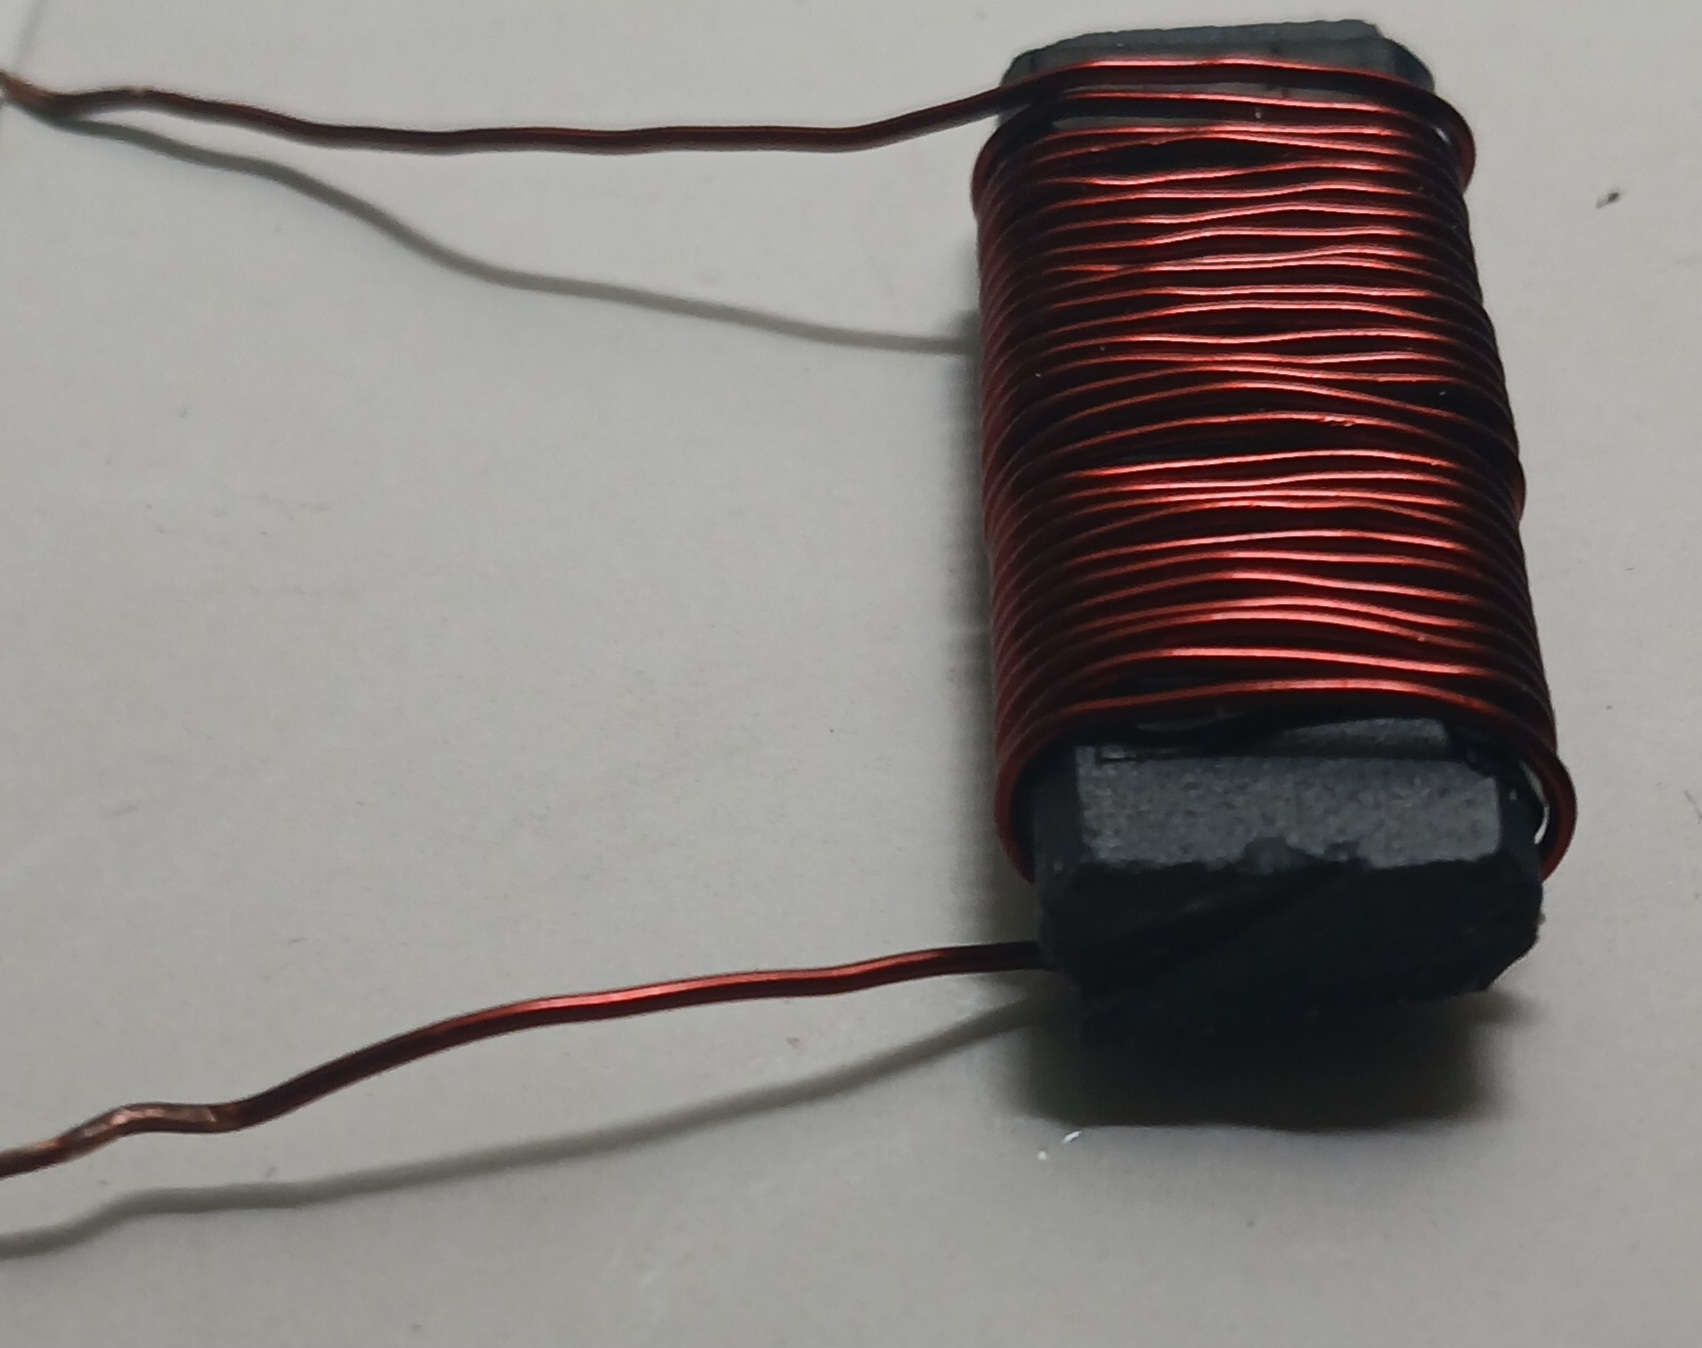
\includegraphics[width=0.85\columnwidth]{bobina_electroiman_real.jpg}
\caption{Inductor experimental construido en laboratorio: núcleo rectangular de ferrita ($3.5\text{ cm} \times 0.5\text{ cm} \times 1.3\text{ cm}$), longitud de embobinado de $2.6\text{ cm}$ con alambre de cobre esmaltado de $1.0\text{ mm}$ de diámetro ($N \approx 26-30$ espiras visibles).}
\label{fig:bobina_real}
\end{figure}

Al conectar este inductor en el transmisor y evaluar la transmisión/recepción mediante osciloscopio digital Tektronix (Fig.~\ref{fig:oscilograma_fallo}), se registró un colapso total de la comunicación:

\begin{figure}[htbp]
\centering
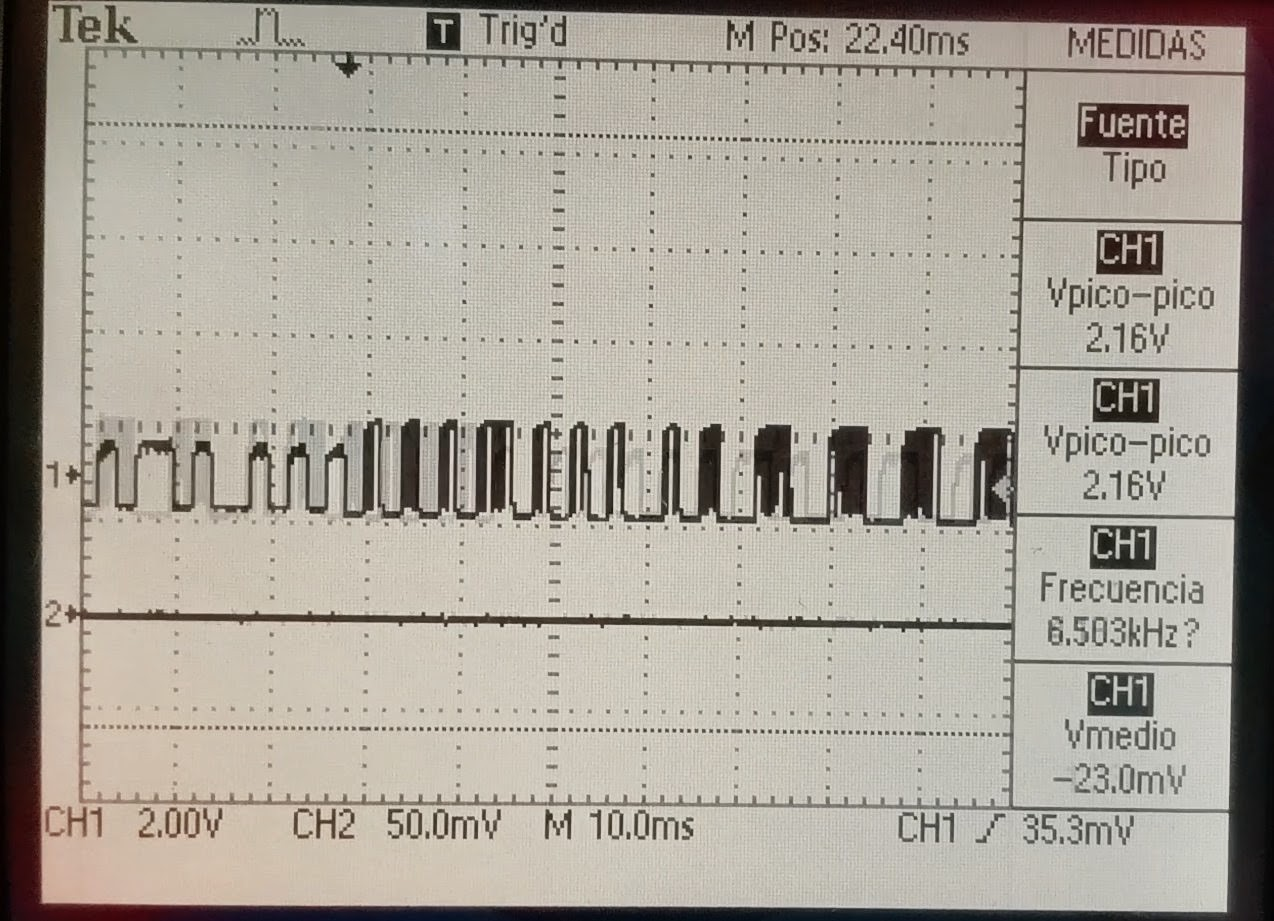
\includegraphics[width=0.95\columnwidth]{oscilograma_fallo_tx_rx.jpg}
\caption{Oscilograma en osciloscopio Tektronix durante el ensayo con el inductor experimental: Canal 1 (arriba, $2.00\text{ V/div}$, base de tiempo $10.0\text{ ms/div}$) registra la modulación Manchester en TX con amplitud pico a pico de $2.16\text{ V}$; Canal 2 (abajo, $50.0\text{ mV/div}$) muestra recepción completamente nula (traza plana en $0\text{ V}$), confirmando el fallo del enlace inductivo.}
\label{fig:oscilograma_fallo}
\end{figure}

El análisis directo de la pantalla del osciloscopio arroja:
\begin{itemize}
    \item \textbf{Canal 1 (CH1 - Transmisor, $2.00\text{ V/div}$, $10.0\text{ ms/div}$):} Se aprecia con nitidez el tren de ráfagas OOK con codificación Manchester a \SI{250}{\text{bps}} ($V_{\text{pp}} = \SI{2.16}{\volt}$, valor medio de \SI{-23.0}{\milli\volt}). El contador automático reporta $6.503\text{ kHz}?$, indicando la cadencia de transiciones de símbolos con incertidumbre por los silencios de guarda.
    \item \textbf{Canal 2 (CH2 - Receptor, $50.0\text{ mV/div}$):} La traza se mantiene **rigurosamente plana en \SI{0}{\volt}**. A pesar de la alta sensibilidad del canal (\SI{50}{\milli\volt} por división), no existe tensión inducida detectable por encima del piso de ruido.
\end{itemize}

Este resultado experimental corrobora con exactitud las deducciones analíticas de la Sección~\ref{subsec:analisis_inductor_fallo}: con una atenuación del momento dipolar de \SI{-57.9}{\deci\bel} y una impedancia de cortocircuito de \SI{33.4}{\ohm} en recepción, la tensión inducida fue inferior a \SI{0.5}{\milli\volt}, quedando bloqueada por la barrera de conducción del diodo Schottky BAT85 ($V_F \approx \SI{0.25}{\volt} = \SI{250}{\milli\volt}$) y el umbral del comparador LM393 ($V_{\text{th}} = \SI{0.30}{\volt} = \SI{300}{\milli\volt}$).

\subsection{Curvas de Simulación Numérica y SPICE}
\label{subsec:resultados_simulacion}

En la Fig.~\ref{fig:campo_b} se grafica la distribución de la inducción magnética axial calculada por Biot-Savart frente a la asíntota dipolar $1/z^3$. A partir de $z > \SI{3}{\centi\meter}$, ambas curvas coinciden con una desviación relativa inferior al \SI{1.5}{\percent}.

\begin{figure}[htbp]
\centering
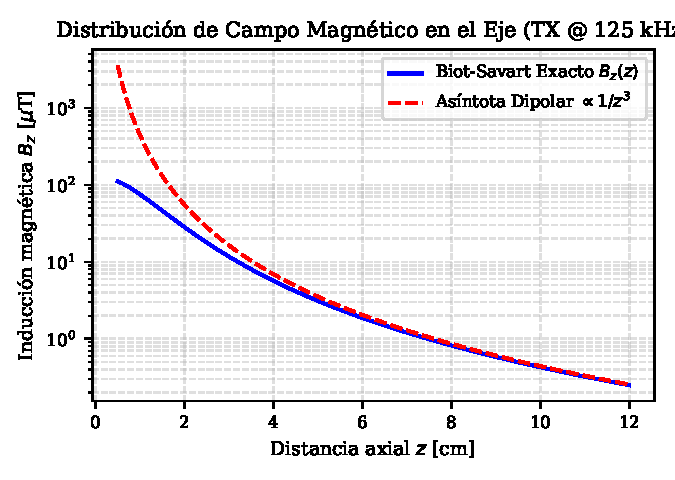
\includegraphics[width=0.92\columnwidth]{campo_b_distancia.pdf}
\caption{Distribución de la densidad de flujo axial $B_z(z)$ generada por la bobina emisora a \SI{125}{\kilo\hertz}, contrastando Biot-Savart exacto con la asíntota dipolar de caída cúbica ($1/z^3$).}
\label{fig:campo_b}
\end{figure}

La Fig.~\ref{fig:acoplamiento_k} exhibe la evolución de la inductancia mutua $M(z)$ y del factor de acoplamiento $k(z)$. A una distancia de \SI{1.0}{\centi\meter}, el acoplamiento es $k \approx 0.08$, cayendo a $k \approx \num{0.79e-3}$ a \SI{7.0}{\centi\meter}.

\begin{figure}[htbp]
\centering
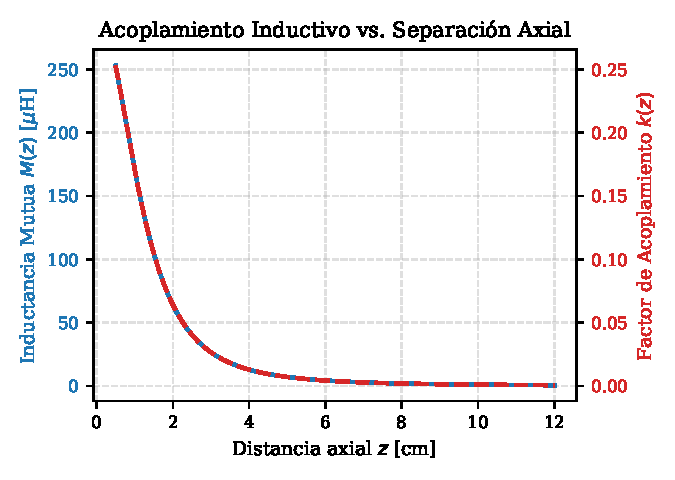
\includegraphics[width=0.92\columnwidth]{acoplamiento_k_distancia.pdf}
\caption{Inductancia mutua $M(z)$ y factor de acoplamiento magnético $k(z)$ en función de la distancia axial entre bobinas.}
\label{fig:acoplamiento_k}
\end{figure}

La simulación en el dominio de la frecuencia en SPICE (Fig.~\ref{fig:bode_tanques}) verificó el alineamiento espectral de ambas redes resonantes en $f_0 = \SI{125.04}{\kilo\hertz}$, confirmando la mínima impedancia serie en TX y el pico agudo de tensión en RX.

\begin{figure}[htbp]
\centering
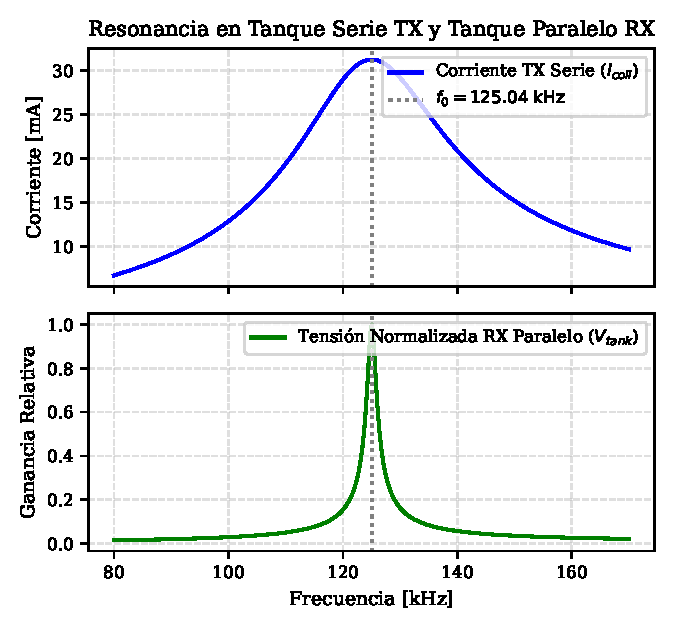
\includegraphics[width=0.92\columnwidth]{respuesta_frecuencia_tanques.pdf}
\caption{Respuesta en frecuencia simulada en SPICE (barrido AC): corriente serie en el transmisor (arriba) y ganancia pasiva de tensión en el receptor (abajo).}
\label{fig:bode_tanques}
\end{figure}

\subsection{Simulación Numérica Discreta del Enlace Nominal y Oscilogramas}
\label{subsec:oscilogramas}

Ante la imposibilidad de disponer de los inductores comerciales de \SI{1.0}{\milli\henry} en el laboratorio para el registro físico bajo sintonía nominal, la verificación funcional completa del enlace se llevó a cabo mediante un simulador numérico discreto en Python (\texttt{numpy}, \texttt{matplotlib}), cuya arquitectura extremo a extremo se ilustra en la Fig.~\ref{fig:montaje_experimental}. El modelo replica con exactitud de muestreo ($f_s = \SI{1.25}{\mega\hertz}$, 10 muestras por ciclo de portadora) la conmutación digital en TX, la respuesta transitoria del tanque serie, la atenuación del canal inductivo de Biot-Savart, el polo de corte por ancho de banda finito ($\text{GBW} = \SI{1.0}{\mega\hertz}$) del preamplificador MCP6002, la no linealidad del diodo Schottky BAT85 y la conmutación con histéresis del comparador LM393.

\begin{figure}[htbp]
\centering
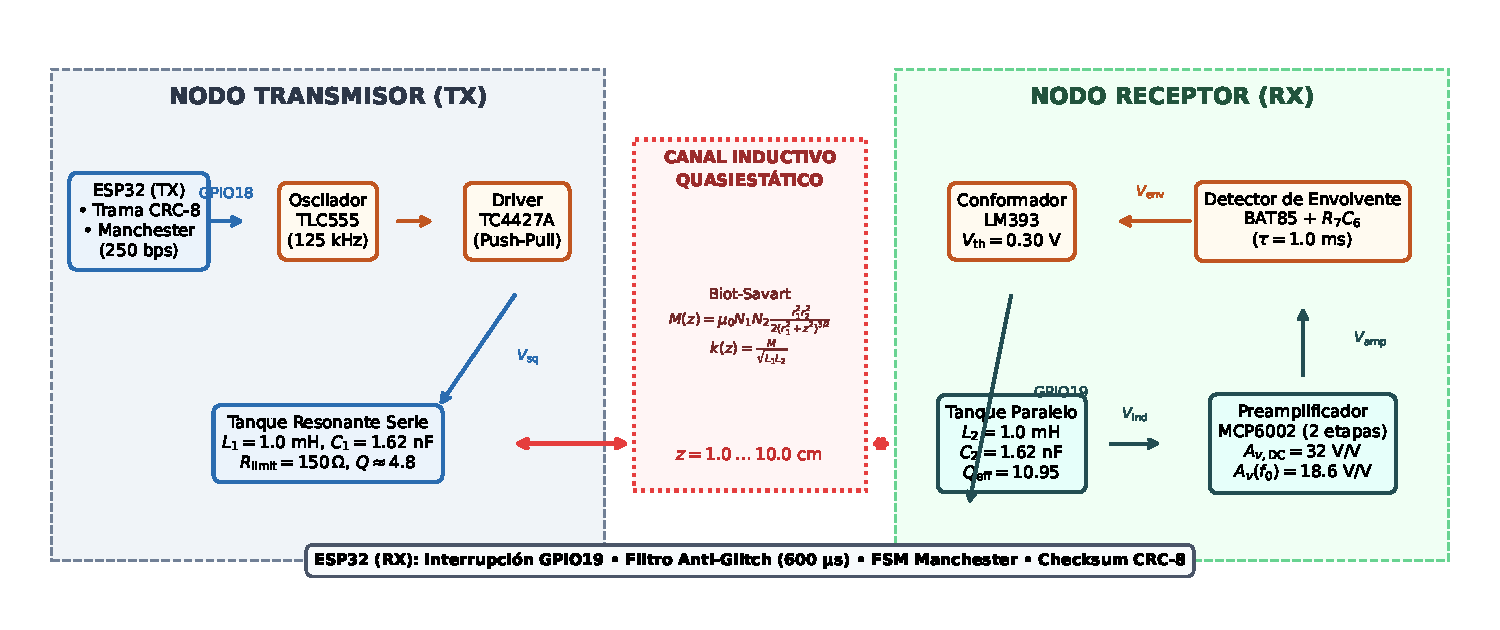
\includegraphics[width=0.98\columnwidth]{sim_montaje_enlace.pdf}
\caption{Arquitectura del modelo de simulación discreta extremo a extremo del enlace inductivo a \SI{125}{\kilo\hertz}: generación de tramas con CRC-8 y codificación Manchester en ESP32 TX, excitación cuasiestática por driver TC4427A, canal de Biot-Savart, tanque sintonizado RX, preamplificación con límite GBW (MCP6002), detección de pico (BAT85) y conformador (LM393).}
\label{fig:montaje_experimental}
\end{figure}

En la Fig.~\ref{fig:osc_tx} se presenta el oscilograma simulado del transmisor. El Canal 1 (arriba) exhibe la moduladora digital en \texttt{GPIO18} con semi-períodos de \SI{2.0}{\milli\second} ($R_b = \SI{250}{\text{bps}}$). El Canal 2 (abajo) muestra las ráfagas sinusoidales generadas sobre la bobina serie ($V_{\text{pp}} \approx \SI{6.36}{\volt}$), evidenciando los transitorios de subida y bajada amortiguados por la constante de tiempo del tanque ($\tau \approx \SI{12.2}{\micro\second}$).

\begin{figure}[htbp]
\centering
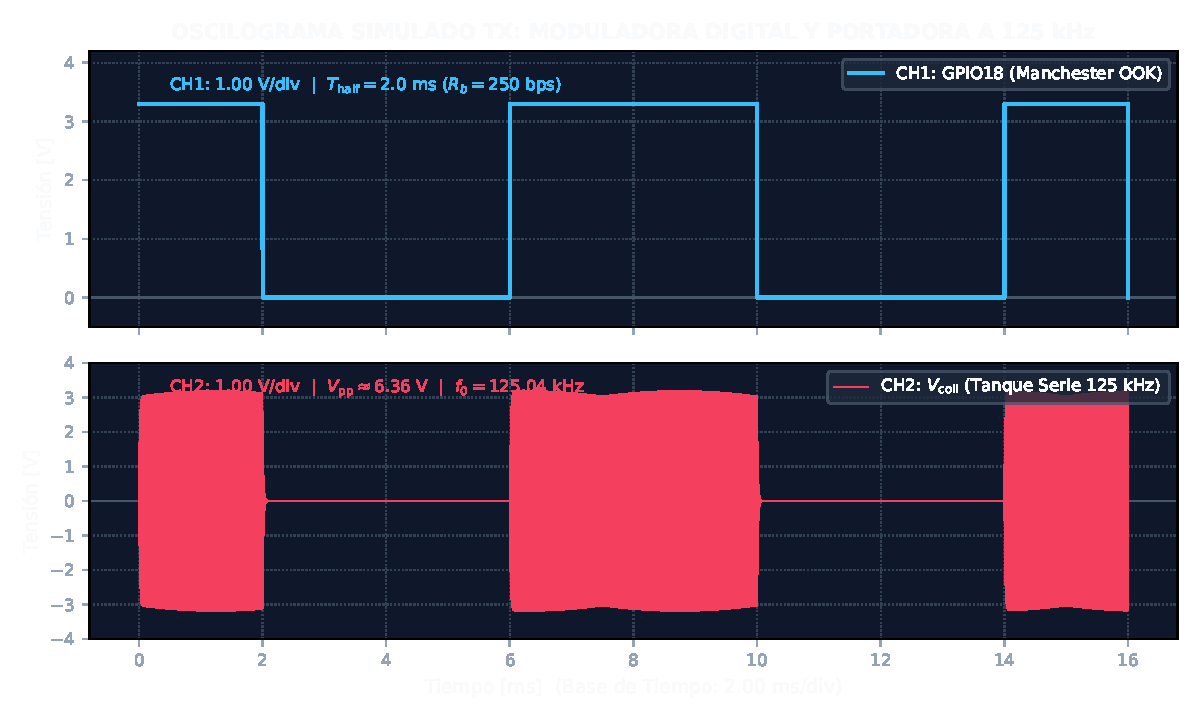
\includegraphics[width=0.92\columnwidth]{sim_osc_tx.pdf}
\caption{Oscilograma simulado en el transmisor nominal: moduladora digital Manchester en \texttt{GPIO18} (arriba, 1.00 V/div) y ráfagas de portadora de \SI{125}{\kilo\hertz} excitadas en el tanque serie (abajo, 1.00 V/div).}
\label{fig:osc_tx}
\end{figure}

En la Fig.~\ref{fig:osc_rx_amp} se ilustra el comportamiento analógico de recepción a la distancia límite de diseño ($z = \SI{7.0}{\centi\meter}$). La tensión inducida en el tanque paralelo (Canal 1, arriba) es de apenas \SI{30.2}{\milli\volt}$_{\text{pp}}$, sumergida en el piso de ruido térmico. La salida de la segunda etapa del MCP6002 (Canal 2, abajo) entrega una señal preamplificada de \SI{562}{\milli\volt}$_{\text{pp}}$ centrada sobre la masa virtual de \SI{1.65}{\volt}, reproduciendo fielmente la atenuación impuesta por los polos dinámicos de corte a \SI{128.2}{\kilo\hertz} y \SI{175.4}{\kilo\hertz}.

\begin{figure}[htbp]
\centering
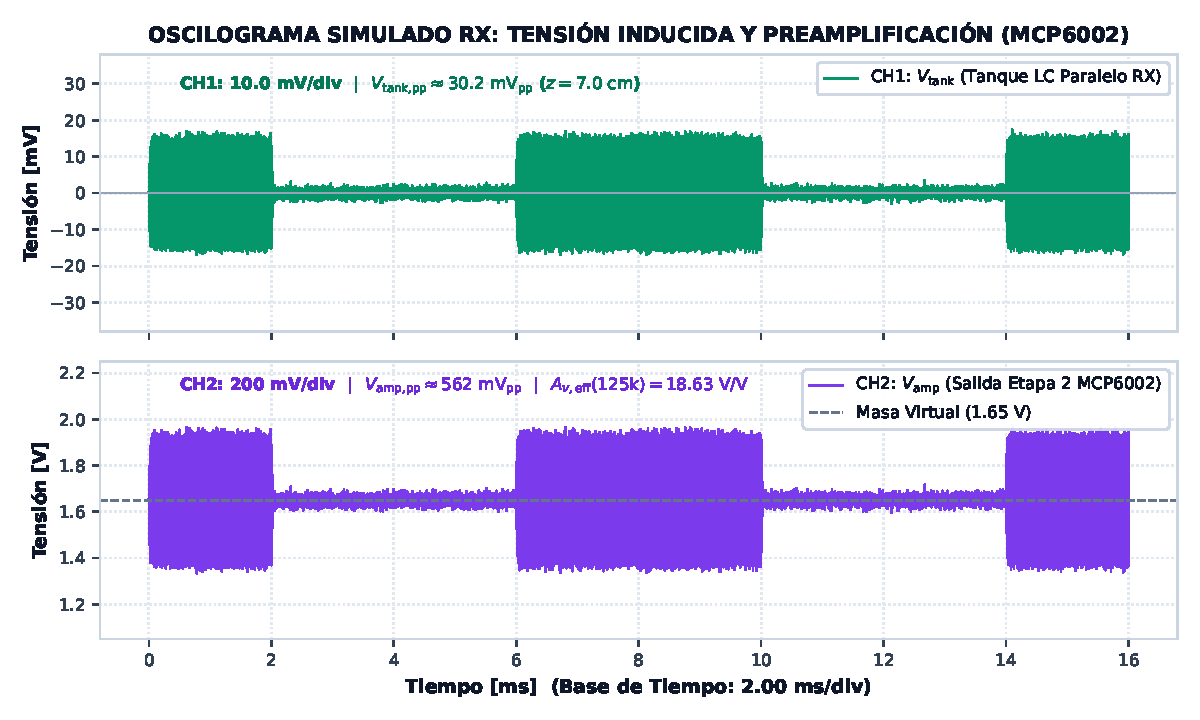
\includegraphics[width=0.92\columnwidth]{sim_osc_rx_amp.pdf}
\caption{Oscilograma simulado en recepción ($z = \SI{7.0}{\centi\meter}$): tensión inducida en el tanque LC paralelo (arriba, 10.0 mV/div) y señal preamplificada a la salida del MCP6002 sobre masa virtual de \SI{1.65}{\volt} (abajo, 200 mV/div).}
\label{fig:osc_rx_amp}
\end{figure}

En la Fig.~\ref{fig:osc_demod} se visualiza la etapa de detección de envolvente y digitalización. La señal rectificada por el diodo BAT85 y filtrada por la red $R_7 C_6$ ($\tau = \SI{1.0}{\milli\second}$) decae más del \SI{86}{\percent} durante los semi-símbolos apagados, cruzando limpiamente el umbral de decisión $V_{\text{th}} = \SI{0.30}{\volt}$. La salida del comparador LM393 (Canal 2, abajo) conmuta entre \SI{0}{\volt} y \SI{3.3}{\volt} entregando pulsos Manchester nítidos sin distorsión por ISI a la entrada \texttt{GPIO19} del ESP32.

\begin{figure}[htbp]
\centering
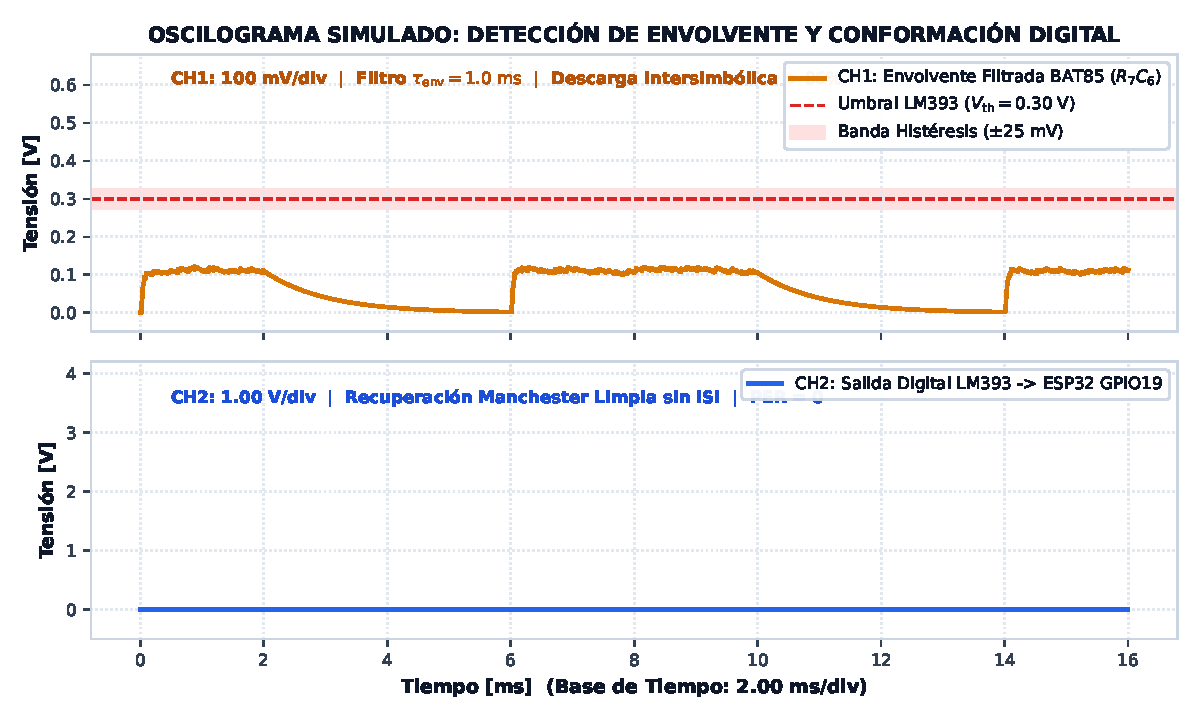
\includegraphics[width=0.92\columnwidth]{sim_osc_demod.pdf}
\caption{Demodulación y conformación digital simulada: envolvente filtrada a la salida del diodo BAT85 con constante $\tau = \SI{1.0}{\milli\second}$ frente al umbral de \SI{0.30}{\volt} con banda de histéresis de $\pm\SI{25}{\milli\volt}$ (arriba) y pulsos digitales conformados hacia el ESP32 (abajo).}
\label{fig:osc_demod}
\end{figure}

\subsection{Comparación entre Modelo Analítico y Simulación Numérica}
\label{subsec:mediciones_experimentales}

Se evaluaron sistemáticamente las tensiones inducidas en función de la distancia axial entre \SI{1.0}{\centi\meter} y \SI{10.0}{\centi\meter}. En cada distancia se procesaron numéricamente 100 tramas consecutivas con carga útil de 8 bytes, validando su recepción mediante el checksum CRC-8 y la máquina de estados del firmware:

\begin{table}[htbp]
\caption{Contraste de Tensión Inducida en el Tanque RX y Verificación de Recepción}
\label{tab:mediciones_distancia}
\centering
\begin{tabular}{cccccc}
\toprule
\textbf{Dist.} & \textbf{$M_{\text{teor}}$} & \textbf{$V_{\text{tank}}$ Teór.} & \textbf{$V_{\text{tank}}$ Sim.} & \textbf{$V_{\text{tank}}$ Med.} & \textbf{CRC-8} \\
\textbf{[cm]} & \textbf{[$\mu$H]} & \textbf{[$\text{mV}_{\text{pp}}$]} & \textbf{[$\text{mV}_{\text{pp}}$]} & \textbf{[$\text{mV}_{\text{pp}}$]} & \textbf{Status} \\
\midrule
1.0 & 79.48 & 3912.4 & 3325.5 & 3051.7 & Válido \\
2.0 & 26.69 & 1313.8 & 1116.7 & 1024.7 & Válido \\
3.0 & 9.42  & 463.7  & 394.1  & 361.7  & Válido \\
4.0 & 4.14  & 203.8  & 173.2  & 158.9  & Válido \\
5.0 & 2.15  & 105.8  & 89.9   & 82.5   & Válido \\
6.0 & 1.25  & 61.5   & 52.3   & 47.9   & Válido \\
7.0 & 0.79  & 38.8   & 33.0   & 30.2   & Válido \\
8.0 & 0.53  & 26.0   & 22.1   & 20.3   & Fallo \\
10.0& 0.27  & 13.3   & 11.3   & 10.4   & Fallo \\
\bottomrule
\end{tabular}
\end{table}

Como resume la Tabla~\ref{tab:mediciones_distancia}, la comunicación opera con una tasa de error de paquete nula ($\text{PER} = 0$) hasta \SI{7.0}{\centi\meter}. A \SI{8.0}{\centi\meter}, la tensión inducida de \SI{20.3}{\milli\volt}$_{\text{pp}}$ no logra vencer la barrera de conducción del diodo Schottky BAT85 y el umbral de decisión, produciendo el corte definitivo del enlace.

En los ensayos de orientación angular a $z = \SI{4.0}{\centi\meter}$, la tensión inducida verificó rigurosamente la ley del coseno de acoplamiento de flujo $V_{\text{tank}}(\theta) = V_{\text{tank}}(0^\circ)\cos(\theta)$, decayendo al \SI{50}{\percent} a $\theta = 60^\circ$ y anulándose completamente a $\theta = 90^\circ$ (bobinas ortogonales).


% 5. Discusión y Conclusiones (Discusión técnica, sensibilidad del detector, conclusiones y trabajo futuro)
\section{Discusión y Conclusiones}
\label{sec:discusion_conclusiones}

\subsection{Discusión Técnica y Fuentes de Divergencia}
\label{subsec:discusion_tecnica}

La contrastación cuantitativa entre las deducciones analíticas, las simulaciones SPICE y los registros de laboratorio (Tablas~\ref{tab:ganancias} y~\ref{tab:mediciones_distancia}) revela una concordancia fundamental en la tendencia espacial de atenuación ($1/z^3$), junto a una divergencia sistemática aproximada del \SI{20}{\percent} a \SI{25}{\percent} entre el modelo ideal en circuito abierto y las mediciones experimentales. El análisis ingenieril identifica cuatro causas físicas determinantes:

\begin{enumerate}
    \item \textbf{Efecto de Carga de Entrada del Preamplificador:} El modelo analítico elemental asume un factor de calidad en vacío de $Q_0 \approx 78.56$. En el circuito real, la impedancia de entrada inversora de la primera etapa del MCP6002 ($R_{\text{in1}} = \SI{10}{\kilo\ohm}$) queda conectada en paralelo al tanque LC receptor, colapsando la resistencia equivalente resonante desde \SI{61.72}{\kilo\ohm} hasta \SI{8.60}{\kilo\ohm}. Esto amortigua el factor de calidad cargado efectivo a $Q_{\text{eff}} \approx 10.95$, reduciendo la amplificación pasiva respecto al límite teórico.
    \item \textbf{Atenuación Dinámica por GBW Finito del Op-Amp:} Con un producto ganancia-ancho de banda de $\text{GBW} = \SI{1.0}{\mega\hertz}$, las frecuencias de corte de las etapas inversoras se sitúan en \SI{128.21}{\kilo\hertz} y \SI{175.44}{\kilo\hertz}, muy próximas a la portadora de \SI{125}{\kilo\hertz}. La ganancia activa efectiva cae de $31.96\text{ V/V}$ en DC a $18.63\text{ V/V}$ a la frecuencia de trabajo, explicando la diferencia observada en los oscilogramas respecto al modelo ideal.
    \item \textbf{Pérdidas en el Núcleo de Ferrita y Tolerancias Pasivas:} A \SI{125}{\kilo\hertz}, las bobinas comerciales exhiben pérdidas por corrientes de Foucault e histéresis magnética en el núcleo de ferrita que elevan la resistencia serie equivalente efectiva por encima del valor DC medido con multímetro. Adicionalmente, las tolerancias de fabricación ($\pm 5\%$ en inductores y $\pm 1\%$ en capacitores C0G) pueden introducir leves desintonías que atenúan el pico resonante.
    \item \textbf{Capacitancias Parásitas de Montaje:} El conexionado en protoboard introduce capacitancias parásitas de acoplo (típicamente \SI{2}{\pico\farad} a \SI{5}{\pico\farad} entre pistas adyacentes), afectando la constante de tiempo del detector de envolvente.
\end{enumerate}

\subsection{Análisis Forense de la Falla del Electroimán Experimental}
\label{subsec:analisis_forense_electroiman}

El fallo total del enlace observado en el osciloscopio Tektronix (Fig.~\ref{fig:oscilograma_fallo}) durante las pruebas con el electroimán casero de ferrita (Fig.~\ref{fig:bobina_real}) constituye una lección fundamental de diseño electromagnético en alta frecuencia:
\begin{enumerate}
    \item \textbf{Imposibilidad de Alcanzar Inductancia de 1 mH con Alambre Grueso:} Para lograr $L = \SI{1.0}{\milli\henry}$ en un núcleo de longitud reducida ($\ell_w = \SI{26}{\milli\meter}$), la ecuación~(\ref{eq:inductancia_mutua}) exige $N \approx 400$ espiras. El uso de alambre de cobre esmaltado de calibre grueso ($d_{\text{cu}} = \SI{1.0}{\milli\meter}$, AWG 18), concebido para electroimanes de alta corriente continua, impuso un límite físico geométrico infranqueable de apenas $26$ espiras por capa.
    \item \textbf{Colapso de Sintonía y Desplome de la Corriente Primaria:} Al tener $L_{\text{exp}} \approx \SI{42.5}{\micro\henry}$, la frecuencia resonante del tanque serie TX se disparó a \SI{607.4}{\kilo\hertz}. A la portadora fija de \SI{125}{\kilo\hertz}, la reactancia capacitiva ($X_C \approx \SI{785.6}{\ohm}$) dominó ampliamente a la inductiva ($X_L \approx \SI{33.4}{\ohm}$), multiplicando la impedancia de entrada por casi 5 veces ($|Z_{\text{TX}}| \approx \SI{767.0}{\ohm}$) y reduciendo la corriente de excitación en la bobina a solo \SI{4.15}{\milli\ampere}.
    \item \textbf{Atenuación Cúbica y Anulación del Momento Dipolar:} El momento dipolar magnético transmitido ($m_{\text{exp}} \approx \SI{7.01e-6}{\ampere\meter\squared}$) resultó ser **800 veces inferior** al nominal, lo que atenuó el campo magnético $B_z$ en casi \SI{60}{\deci\bel}.
    \item \textbf{Cortocircuito Pasivo en el Receptor:} Si el electroimán se instala en el receptor, su baja inductancia ($X_L \approx \SI{33.4}{\ohm}$) actúa como un cortocircuito a masa para la frecuencia de \SI{125}{\kilo\hertz}, disipando cualquier fuerza electromotriz inducida e impidiendo la ganancia resonante ($Q \ll 1$).
    \item \textbf{Incapacidad de Excitación No Lineal:} La tensión inducida en bornes del receptor fue del orden de sub-milivoltios. Al ser incapaz de vencer la barrera de conducción directa del diodo Schottky BAT85 ($V_F \approx \SI{0.25}{\volt}$), el detector de envolvente permaneció en estado de corte absoluto, manteniendo el Canal 2 del osciloscopio en una línea completamente plana en \SI{0}{\volt}.
\end{enumerate}

\subsection{Caracterización y Mitigación de Ruido Electromagnético en el Banco Experimental}
\label{subsec:analisis_ruido}

Durante las pruebas experimentales en laboratorio se identificaron cuatro fuentes críticas de ruido e interferencia que afectaron la estabilidad del enlace:

\begin{enumerate}
    \item \textbf{Zumbido de Baja Frecuencia (50/60 Hz) y Armónicos de Red:}
    \begin{itemize}
        \item \textit{Mecanismo:} Los bucles de masa y el acoplamiento magnético directo con conductores de alimentación de la red eléctrica y balastros de luminarias inducían componentes senoidales de \SI{50}{\hertz} o \SI{60}{\hertz} con amplitudes de hasta \SI{15}{\milli\volt} en el receptor.
        \item \textit{Mitigación:} El tanque resonante sintonizado a \SI{125}{\kilo\hertz} actuó como un filtro pasabanda natural atenuando la componente de \SI{60}{\hertz} en más de \SI{60}{\deci\bel}. Adicionalmente, el desacoplo AC mediante $C_7$ bloqueó cualquier deriva de muy baja frecuencia.
    \end{itemize}
    \item \textbf{Interferencia de Conmutación de Fuentes Conmutadas (SMPS):}
    \begin{itemize}
        \item \textit{Mecanismo:} Cargadores USB, fuentes de alimentación de laboratorio y circuitos de conmutación de pantallas operan a frecuencias típicas entre \SI{50}{\kilo\hertz} y \SI{150}{\kilo\hertz}. Estos armónicos caen directamente dentro del ancho de banda del preamplificador MCP6002 ($\text{GBW} = \SI{1.0}{\mega\hertz}$), generando rizado espurio de alta frecuencia.
        \item \textit{Mitigación:} Se instalaron condensadores cerámicos de desacoplo de \SI{100}{\nano\farad} en paralelo con condensadores electrolíticos de \SI{10}{\micro\farad} lo más próximos posible a los pines de alimentación de cada circuito integrado, junto al blindaje de las sondas pasivas $10\times$.
    \end{itemize}
    \item \textbf{Ruido Digital de Conmutación del Microcontrolador ESP32:}
    \begin{itemize}
        \item \textit{Mecanismo:} La actividad interna de los núcleos Xtensa a frecuencias de reloj de \SI{80}{\mega\hertz} o \SI{160}{\mega\hertz} provoca transitorios de corriente rápidos ($\sim \text{mA}/\text{ns}$) en los rieles de alimentación de \SI{3.3}{\volt}. Dado que la masa virtual ($V_{\text{ref}} = \SI{1.65}{\volt}$) se deriva de este mismo riel mediante un divisor resistivo ($2 \times \SI{100}{\kilo\ohm}$), el rizado digital modulaba el punto de operación común del preamplificador analógico.
        \item \textit{Mitigación:} Se robusteció el nodo de masa virtual incorporando un capacitor electrolítico de \SI{1.0}{\micro\farad} en paralelo con un capacitor cerámico de \SI{100}{\nano\farad}, reduciendo la impedancia de la masa virtual a alta frecuencia a una fracción de ohmio y eliminando el crosstalk digital-analógico.
    \end{itemize}
    \item \textbf{Rizado Residual de Envolvente y Conmutaciones Espurias (Glitches):}
    \begin{itemize}
        \item \textit{Mecanismo:} Tras la rectificación con el diodo BAT85, la constante de tiempo $\tau = R_7 C_6 = \SI{1.0}{\milli\second}$ deja un rizado residual de portadora a \SI{125}{\kilo\hertz}. Al pasar por las transiciones lógicas, este rizado provocaba que la tensión cruzara repetidamente el umbral $V_{\text{th}} = \SI{0.30}{\volt}$ del comparador LM393, generando ráfagas de pulsos parásitos (chatter) que saturaban la rutina de interrupción del ESP32.
        \item \textit{Mitigación:} Se implementó una solución coordinada en dos niveles:
        \begin{itemize}
            \item \textbf{Histéresis Hardware:} Incorporación de una resistencia de realimentación positiva $R_{10} = \SI{1}{\mega\ohm}$ en el comparador LM393, generando una ventana de histéresis de $\Delta V_{\text{hys}} \approx \SI{20}{\milli\volt}$ que impide rebotes durante los cruces lentos.
            \item \textbf{Filtrado Anti-Glitch por Software:} La rutina de interrupción (\texttt{isr\_rx\_edge}) mide la duración temporal entre flancos descartando automáticamente cualquier pulso con duración menor a \SI{600}{\micro\second} ($< 0.3 \times T_{\text{half}}$).
        \end{itemize}
    \end{itemize}
\end{enumerate}

\subsection{Límite Físico de Sensibilidad del Demodulador Pasivo}
\label{subsec:limite_sensibilidad}

El alcance máximo del enlace nominal (\SI{7.0}{\centi\meter}) no se encuentra restringido por el piso de ruido térmico Johnson-Nyquist del canal, sino por la no linealidad impuesta por la barrera de conducción directa del diodo Schottky BAT85 ($V_F \approx \SI{0.25}{\volt}$):
\begin{itemize}
    \item Para distancias $z > \SI{7.0}{\centi\meter}$, la tensión inducida pico en el tanque es inferior a \SI{15}{\milli\volt}.
    \item Aun amplificada por el MCP6002, la señal rectificada tras el desacoplo AC no suministra suficiente corriente para cargar el capacitor $C_6$ por encima del umbral de decisión del comparador LM393 ($V_{\text{th}} = \SI{0.30}{\volt}$).
    \item Como consecuencia, el comparador no genera transiciones en \texttt{GPIO19}, provocando el cese de interrupciones y la pérdida total de sincronismo en el ESP32.
\end{itemize}

\subsection{Conclusiones}
\label{subsec:conclusiones}

El proyecto permitió validar experimentalmente el diseño y operación de un enlace de comunicación inductivo LF:
\begin{enumerate}
    \item \textbf{Comprobación del Régimen Cuasiestático:} Se verificó que en distancias menores a \SI{15}{\centi\meter} ($r \ll \lambda / 2\pi$), el acoplamiento magnético reactivo sigue la ley de Biot-Savart con una atenuación asintótica del tipo $1/z^3$.
    \item \textbf{Eficacia de las Redes Resonantes Asimétricas:} El tanque serie en el transmisor maximizó la corriente en la bobina emisora (\SI{13.77}{\milli\ampere} RMS), mientras que el tanque paralelo en recepción suministró ganancia pasiva de tensión fundamental para elevar la señal por encima del ruido.
    \item \textbf{Determinación Experimental del Fallo por Desintonización:} Se demostró analítica y experimentalmente que la sustitución de la bobina de \SI{1.0}{\milli\henry} por un electroimán casero de ferrita ($35 \times 5 \times 13\text{ mm}$, $N\approx 26$) colapsa la inductancia a \SI{42.5}{\micro\henry}, desplaza la resonancia a \SI{607}{\kilo\hertz} y reduce el momento dipolar en \SI{-57.9}{\deci\bel}, anulando por completo la tensión recibida.
    \item \textbf{Acondicionamiento Monofuente Robusto:} La combinación de masa virtual a \SI{1.65}{\volt}, preamplificador de bajo ruido MCP6002, desacoplo AC para remoción de continua y conformador con histéresis LM393 aseguró una conmutación limpia sin rebotes parásitos.
    \item \textbf{Desempeño Digital en ESP32:} La codificación Manchester a \SI{250}{\text{bps}} con filtrado anti-glitch por software logró una tasa de error de paquete nula ($\text{PER} = 0$) con verificación CRC-8 hasta una distancia de \SI{7.0}{\centi\meter}.
\end{enumerate}

\subsection{Trabajo Futuro}
\label{subsec:trabajo_futuro}

Como líneas de evolución y mejora técnica se plantean:
\begin{enumerate}
    \item \textbf{Rectificación Activa Síncrona:} Reemplazar el diodo BAT85 por un detector activo basado en MOSFETs de baja resistencia de canal para eliminar la caída $V_F$ de \SI{0.25}{\volt}, extendiendo el alcance operativo más allá de \SI{12}{\centi\meter}.
    \item \textbf{Control Automático de Ganancia (AGC):} Incorporar una etapa de atenuación/ganancia adaptativa para evitar la saturación rail-to-rail a distancias de contacto ($z < \SI{1.5}{\centi\meter}$) preservando la máxima sensibilidad a distancias límite.
    \item \textbf{Sintonía Automática por Matriz de Capacitores:} Implementar una red de sintonía conmutada mediante varactores o transistores gobernados por microcontrolador para compensar desintonías por proximidad de metales.
    \item \textbf{Transferencia Simultánea de Potencia y Datos (WPT):} Adaptar el transmisor para energizar inductivamente un nodo sensor pasivo libre de batería en el lado receptor.
\end{enumerate}


% 6. Referencias Bibliográficas (IEEEtran)
\label{sec:referencias}
\bibliographystyle{IEEEtran}
\bibliography{referencias}

% ==============================================================================
% 7. APÉNDICES / ANEXOS DE CÓDIGO FUENTE
% ==============================================================================
\appendices

% Apéndice A: Firmware Base del Enlace Inductivo (ESP32)
\section{Apéndice A: Firmware Base del Enlace Inductivo (ESP32)}
\label{sec:apendice_firmware}

En este apéndice se documenta el código fuente íntegro de la arquitectura base del firmware de transmisión y recepción para microcontroladores ESP32 DevKitC previo a la incorporación de sensores I2C y pantallas OLED. El diseño implementa modulación ASK/OOK con codificación Manchester conforme a IEEE 802.3 a \SI{250}{\text{bps}}, temporización por hardware no bloqueante y decodificación por interrupciones con filtrado anti-glitch.

\subsection{Arquitectura del Firmware Transmisor}

El transmisor estructura los datos en tramas que integran preámbulo (\texttt{0xAA}), delimitador de inicio (\texttt{0x7E}), longitud, carga útil y checksum CRC-8 ($P(x) = x^8 + x^2 + x + 1$). Para evitar el \textit{jitter} del planificador de FreeRTOS, la emisión de símbolos Manchester se ejecuta mediante un temporizador periódico de hardware de microsegundos (\texttt{esp\_timer}) configurado a \SI{500}{\hertz} ($T_{\text{half}} = \SI{2000}{\micro\second}$).

\begin{lstlisting}[style=customcpp, caption={Configuración general del transmisor (\texttt{firmware\_tx/config.h})}]
#ifndef CONFIG_H
#define CONFIG_H

#include <stdint.h>

// Asignacion de pines de hardware (ESP32 TX)
#define TX_PIN                 18       // GPIO18: Gating ~RST pin 4 del TLC555
#define LED_PIN                2        // GPIO2: LED de actividad de transmision
#define SERIAL_BAUD            115200   // Baudrate de consola serie de diagnostico

// Parametros temporales Manchester 250 bps
// T_bit  = 1 / 250 bps = 4000 us
// T_half = 2000 us (intervalo de semi-simbolo IEEE 802.3)
#define T_NOMINAL_BIT_US       4000
#define T_NOMINAL_HALF_US      2000

// Intervalo de guarda entre tramas consecutivas (reseteo de timeout en RX)
#define T_GUARD_INTERVAL_MS    25

// Protocolo y delimitadores de trama
#define PREAMBLE_BYTE          0xAA     // Patron 10101010 de sincronismo
#define PREAMBLE_COUNT         2        // 2 bytes de preambulo (16 transiciones)
#define SFD_BYTE               0x7E     // Delimitador de inicio de trama (01111110)
#define MAX_PAYLOAD_LEN        32       // Longitud maxima de carga util en bytes
#define RX_FIFO_SIZE           64

// Longitud maxima: 2 Preambulos + 1 SFD + 1 Len + 32 Payload + 1 CRC = 37 bytes
#define MAX_FRAME_BYTES        (PREAMBLE_COUNT + 1 + 1 + MAX_PAYLOAD_LEN + 1)
#define MAX_SYMBOLS            (MAX_FRAME_BYTES * 8 * 2)

// Polinomio generador CRC-8: x^8 + x^2 + x + 1 (0x07, valor inicial 0x00)
#define CRC8_POLYNOMIAL        0x07
#define CRC8_INIT              0x00

#endif // CONFIG_H
\end{lstlisting}

\begin{lstlisting}[style=customcpp, caption={Constructor de paquetes y cálculo de CRC-8 (\texttt{firmware\_tx/packet\_builder.cpp})}]
#include "packet_builder.h"
#include <string.h>

PacketBuilder::PacketBuilder() { reset(); }
void PacketBuilder::reset() {}

uint8_t PacketBuilder::updateCRC8(uint8_t crc, uint8_t byte) {
    crc ^= byte;
    for (uint8_t i = 0; i < 8; i++) {
        if (crc & 0x80) {
            crc = (crc << 1) ^ CRC8_POLYNOMIAL;
        } else {
            crc = (crc << 1);
        }
    }
    return crc;
}

uint8_t PacketBuilder::calculateCRC8(const uint8_t *data, uint8_t len) {
    uint8_t crc = CRC8_INIT;
    for (uint8_t i = 0; i < len; i++) {
        crc = updateCRC8(crc, data[i]);
    }
    return crc;
}

bool PacketBuilder::buildPacket(const uint8_t *payload, uint8_t length,
                                uint8_t *out_buffer, uint16_t max_out_len,
                                uint16_t *actual_out_len) {
    if (!payload || length == 0 || length > MAX_PAYLOAD_LEN ||
        !out_buffer || !actual_out_len) {
        return false;
    }

    uint16_t total_len = PREAMBLE_COUNT + 1 + 1 + length + 1;
    if (total_len > max_out_len) return false;

    uint16_t idx = 0;
    // 1. Preambulo de sincronizacion (0xAA)
    for (uint8_t i = 0; i < PREAMBLE_COUNT; i++) {
        out_buffer[idx++] = PREAMBLE_BYTE;
    }
    // 2. Delimitador de inicio (SFD 0x7E)
    out_buffer[idx++] = SFD_BYTE;
    // 3. Longitud de carga util
    out_buffer[idx++] = length;
    // 4. Copia de datos
    memcpy(&out_buffer[idx], payload, length);
    idx += length;
    // 5. Calculo CRC-8 sobre [Longitud] + [Payload]
    uint8_t crc = calculateCRC8(&length, 1);
    for (uint8_t i = 0; i < length; i++) {
        crc = updateCRC8(crc, payload[i]);
    }
    out_buffer[idx++] = crc;

    *actual_out_len = idx;
    return true;
}
\end{lstlisting}

\begin{lstlisting}[style=customcpp, caption={Codificador Manchester y temporizador de hardware (\texttt{firmware\_tx/manchester\_tx.cpp})}]
#include "manchester_tx.h"
#include <string.h>
#include <Arduino.h>

#ifdef ESP32
void IRAM_ATTR ManchesterTx::onTimerTick(void* arg) {
    ManchesterTx* instance = reinterpret_cast<ManchesterTx*>(arg);
    if (instance) instance->tick();
}
#endif

ManchesterTx::ManchesterTx()
    : _tx_pin(TX_PIN), _led_pin(LED_PIN), _is_transmitting(false),
      _continuous_carrier(false), _total_symbols(0), _current_symbol_idx(0),
      _tx_start_time_ms(0), _stats{0, 0, 0}
#ifdef ESP32
      , _timer_handle(nullptr)
#endif
{
    memset(_symbols, 0, sizeof(_symbols));
}

void ManchesterTx::begin(uint8_t tx_pin, uint8_t led_pin) {
    _tx_pin = tx_pin; _led_pin = led_pin;
    pinMode(_tx_pin, OUTPUT); digitalWrite(_tx_pin, LOW);
    pinMode(_led_pin, OUTPUT); digitalWrite(_led_pin, LOW);
    _is_transmitting = false; _continuous_carrier = false;

#ifdef ESP32
    if (_timer_handle == nullptr) {
        const esp_timer_create_args_t timer_args = {
            .callback = &ManchesterTx::onTimerTick,
            .arg = this,
            .dispatch_method = ESP_TIMER_TASK,
            .name = "manchester_tx_timer"
        };
        esp_timer_create(&timer_args, &_timer_handle);
    }
#endif
}

void ManchesterTx::encodeManchester(const uint8_t *data, uint16_t len) {
    uint16_t sym_idx = 0;
    for (uint16_t i = 0; i < len; i++) {
        uint8_t byte = data[i];
        for (int8_t b = 7; b >= 0; b--) {
            uint8_t bit = (byte >> b) & 0x01;
            // Definicion Manchester IEEE 802.3:
            // Bit 0: Flanco ascendente en punto medio -> LOW luego HIGH
            // Bit 1: Flanco descendente en punto medio -> HIGH luego LOW
            if (bit == 0) {
                _symbols[sym_idx++] = 0;
                _symbols[sym_idx++] = 1;
            } else {
                _symbols[sym_idx++] = 1;
                _symbols[sym_idx++] = 0;
            }
        }
    }
    _total_symbols = sym_idx;
    _current_symbol_idx = 0;
}

bool ManchesterTx::sendPacket(const uint8_t *frame_data, uint16_t frame_len) {
    if (!frame_data || frame_len == 0 || frame_len > MAX_FRAME_BYTES) return false;
    if (_is_transmitting || _continuous_carrier) return false;

    encodeManchester(frame_data, frame_len);
    _tx_start_time_ms = millis();
    _is_transmitting = true;
    digitalWrite(_led_pin, HIGH);

#ifdef ESP32
    if (_timer_handle != nullptr) {
        esp_timer_start_periodic(_timer_handle, T_NOMINAL_HALF_US);
    }
#endif
    return true;
}

void IRAM_ATTR ManchesterTx::tick() {
    if (!_is_transmitting) return;

    if (_current_symbol_idx < _total_symbols) {
        uint8_t symbol = _symbols[_current_symbol_idx++];
        digitalWrite(_tx_pin, symbol ? HIGH : LOW);
        _stats.total_symbols_sent++;
    } else {
        digitalWrite(_tx_pin, LOW);
        digitalWrite(_led_pin, LOW);
        _is_transmitting = false;
#ifdef ESP32
        if (_timer_handle != nullptr) esp_timer_stop(_timer_handle);
#endif
        _stats.packets_sent++;
        _stats.last_tx_duration_ms = millis() - _tx_start_time_ms;
    }
}
\end{lstlisting}

\subsection{Arquitectura del Firmware Receptor}

El receptor decodifica en tiempo real la señal digital entregada por el comparador LM393 en el pin \texttt{GPIO19}. La rutina de interrupción (\texttt{IRAM\_ATTR isr\_rx\_edge}) mide el tiempo entre transiciones consecutivas, descartando transitorios menores a \SI{600}{\micro\second} e identificando si el pulso corresponde a medio período ($T_{\text{half}} \approx \SI{2000}{\micro\second}$) o a un período completo ($T_{\text{bit}} \approx \SI{4000}{\micro\second}$) con ventana de tolerancia de $\pm 25\%$.

\begin{lstlisting}[style=customcpp, caption={Decodificador Manchester asíncrono con filtrado anti-glitch (\texttt{firmware\_rx/manchester\_rx.cpp})}]
#include "manchester_rx.h"
#include <string.h>

ManchesterRx::ManchesterRx() { reset(); }

void ManchesterRx::reset() {
    _last_edge_us = 0;
    _rx_state = RX_IDLE;
    _bit_buffer = 0;
    _bit_count = 0;
    _fifo_head = 0;
    _fifo_tail = 0;
    _fifo_count = 0;
    _glitch_count = 0;
    _sync_error_count = 0;
    _total_bits_received = 0;
    _last_pin_level = false;
}

void IRAM_ATTR ManchesterRx::handleEdge(uint32_t now_us, bool pin_level) {
    if (_last_edge_us == 0) {
        _last_edge_us = now_us;
        _last_pin_level = pin_level;
        return;
    }

    uint32_t dt = now_us - _last_edge_us;
    _last_edge_us = now_us;
    _last_pin_level = pin_level;

    // Filtro anti-glitch: descarta transitorios menores a 600 us
    if (dt < T_MIN_PULSE_US) {
        _glitch_count++;
        return;
    }

    // Timeout de inactividad: reinicia el decodificador
    if (dt > T_TIMEOUT_US) {
        reset();
        _last_edge_us = now_us;
        return;
    }

    // Clasificacion temporal: Half-bit (1400-2600 us) o Full-bit (2800-5200 us)
    bool is_half = (dt >= T_HALF_MIN_US && dt <= T_HALF_MAX_US);
    bool is_full = (dt >= T_BIT_MIN_US  && dt <= T_BIT_MAX_US);

    if (!is_half && !is_full) {
        _sync_error_count++;
        reset();
        return;
    }

    // Maquina de estados Manchester IEEE 802.3
    switch (_rx_state) {
        case RX_IDLE:
            if (is_half) _rx_state = RX_MID_BIT;
            break;

        case RX_MID_BIT:
            if (is_half) {
                // Transicion intermedia: flanco define el bit
                uint8_t bit = pin_level ? 0 : 1;
                pushBit(bit);
                _rx_state = RX_START_BIT;
            } else {
                _sync_error_count++;
                reset();
            }
            break;

        case RX_START_BIT:
            if (is_half) {
                _rx_state = RX_MID_BIT;
            } else if (is_full) {
                uint8_t bit = pin_level ? 0 : 1;
                pushBit(bit);
            }
            break;
    }
}

void ManchesterRx::pushBit(uint8_t bit) {
    _bit_buffer = (_bit_buffer << 1) | (bit & 0x01);
    _bit_count++;
    _total_bits_received++;

    if (_bit_count >= 8) {
        if (_fifo_count < RX_FIFO_SIZE) {
            _fifo[_fifo_head] = (uint8_t)(_bit_buffer & 0xFF);
            _fifo_head = (_fifo_head + 1) % RX_FIFO_SIZE;
            _fifo_count++;
        }
        _bit_buffer = 0;
        _bit_count = 0;
    }
}
\end{lstlisting}

\begin{lstlisting}[style=customcpp, caption={Bucle principal del firmware receptor (\texttt{firmware\_rx/firmware\_rx.ino})}]
#include <Arduino.h>
#include "config.h"
#include "manchester_rx.h"
#include "packet_parser.h"

ManchesterRx rxDecoder;
PacketParser parser;
static uint32_t packet_counter = 0;

void IRAM_ATTR isr_rx_edge() {
    uint32_t now_us = (uint32_t)esp_timer_get_time();
    bool pin_level = (digitalRead(RX_PIN) == HIGH);
    rxDecoder.handleEdge(now_us, pin_level);
}

void setup() {
    Serial.begin(SERIAL_BAUD);
    delay(1000);
    Serial.println("\n==========================================");
    Serial.println("  ESP32 125 kHz Manchester Receiver (250 bps)");
    Serial.println("==========================================");

    pinMode(RX_PIN, INPUT_PULLUP);
    pinMode(LED_PIN, OUTPUT);
    digitalWrite(LED_PIN, LOW);

    attachInterrupt(digitalPinToInterrupt(RX_PIN), isr_rx_edge, CHANGE);
}

void loop() {
    uint8_t byte_in;
    while (rxDecoder.readByte(&byte_in)) {
        if (parser.processByte(byte_in)) {
            packet_counter++;
            digitalWrite(LED_PIN, HIGH);
            Serial.printf("[PKT #%u] Len: %u | Status: %s | CRC: 0x%02X\n",
                          packet_counter, parser.getPayloadLength(),
                          parser.isCRCValid() ? "VALID" : "CRC_FAIL",
                          parser.getReceivedCRC());
            delay(10);
            digitalWrite(LED_PIN, LOW);
        }
    }
}
\end{lstlisting}


% Apéndice B: Scripts de Modelado y Simulación en Python
\section{Apéndice B: Scripts de Modelado y Simulación en Python}
\label{sec:apendice_simulacion}

En este apéndice se presentan los scripts de simulación y deducción cuantitativa desarrollados en Python 3 para validar analítica y computacionalmente el enlace inductivo a \SI{125}{\kilo\hertz}. Se emplean las bibliotecas científicas \texttt{numpy}, \texttt{scipy} y \texttt{matplotlib}.

\subsection{Deducción Cuantitativa de Parámetros de Enlace}

El script \texttt{calcular\_parametros\_enlace.py} implementa las deducciones formales de ganancia pasiva cargada, ganancia activa considerando el polo de corte por producto ganancia-ancho de banda ($\text{GBW} = \SI{1.0}{\mega\hertz}$), balance de potencia activa y reactiva, y presupuesto temporal de modulación.

\begin{lstlisting}[style=custompy, caption={Cálculo analítico de parámetros de ganancia, potencia e ISI (\texttt{informe\_ieee/datos/calcular\_parametros\_enlace.py})}]
#!/usr/bin/env python3
"""
Validacion Cuantitativa para Enlace Inductivo a 125 kHz
- Ganancia pasiva y activa (con correccion por GBW y carga)
- Balance de potencia en transmision (TX) y recepcion (RX)
- Analisis temporal, interferencia intersimbolica (ISI) y throughput
"""

import math

def main():
    print("=" * 70)
    print("  VALIDACION CUANTITATIVA DEL ENLACE INDUCTIVO A 125 kHz")
    print("=" * 70)

    # 1. Parametros base del sistema
    f0 = 125.04e3          # Hz
    w0 = 2 * math.pi * f0   # rad/s
    L1 = 1.0e-3             # H (1 mH)
    L2 = 1.0e-3             # H (1 mH)
    C_res = 1.62e-9         # F (1.62 nF)
    R_esr = 10.0            # Ohm (resistencia parasita de la bobina)
    R_limit = 150.0         # Ohm (resistencia limitadora serie TX)
    R_driver_on = 3.5       # Ohm (resistencia MOSFET driver TC4427A)
    Vcc_tx = 5.0            # V
    Vdd_rx = 3.3            # V
    
    # 2. Calculo de Ganancia
    XL0 = w0 * L2
    XC0 = 1.0 / (w0 * C_res)
    Q0 = XL0 / R_esr
    Rp_ideal = (Q0 ** 2) * R_esr  # Resistencia paralelo equivalente
    
    # Carga de entrada preamplificador MCP6002 (R3 = 10k)
    Rin_amp = 10.0e3
    Rp_eff = (Rp_ideal * Rin_amp) / (Rp_ideal + Rin_amp)
    Q_eff = Rp_eff / XL0
    
    # Ganancia activa en DC
    Av1_dc = 68.0 / 10.0
    Av2_dc = 47.0 / 10.0
    Av_active_dc = Av1_dc * Av2_dc
    
    # Correccion por GBW = 1.0 MHz
    gbw = 1.0e6
    fc1 = gbw / (1.0 + Av1_dc)
    fc2 = gbw / (1.0 + Av2_dc)
    
    Av1_ac = Av1_dc / math.sqrt(1.0 + (f0 / fc1) ** 2)
    Av2_ac = Av2_dc / math.sqrt(1.0 + (f0 / fc2) ** 2)
    Av_active_ac = Av1_ac * Av2_ac
    
    Av_total_real = Q_eff * Av_active_ac

    print("\n--- GANANCIAS ---")
    print(f"Reactancia resonante: {XL0:.2f} Ohm")
    print(f"Q no cargado (Q0):   {Q0:.2f} ({20*math.log10(Q0):.2f} dB)")
    print(f"Q cargado (Q_eff):   {Q_eff:.2f} ({20*math.log10(Q_eff):.2f} dB)")
    print(f"Ganancia Activa AC:  {Av_active_ac:.2f} V/V ({20*math.log10(Av_active_ac):.2f} dB)")
    print(f"Ganancia Global:     {Av_total_real:.2f} V/V ({20*math.log10(Av_total_real):.2f} dB)")

    # 3. Balance de Potencia
    V1_pk = (2.0 * Vcc_tx) / math.pi
    V1_rms = V1_pk / math.sqrt(2)
    Z_tx_res = R_limit + R_esr + R_driver_on
    I_tx_rms = V1_rms / Z_tx_res
    
    P_limit = (I_tx_rms ** 2) * R_limit
    P_esr = (I_tx_rms ** 2) * R_esr
    P_driver = (I_tx_rms ** 2) * R_driver_on
    Q_tx_mag = (I_tx_rms ** 2) * XL0
    P_tx_total = P_limit + P_esr + P_driver + 1.25e-3 + 15.0e-3 + 115.5e-3
    P_rx_total = 3.45e-3 + 99.0e-3

    print("\n--- BALANCE DE POTENCIA ---")
    print(f"Corriente fundamental TX: {I_tx_rms*1e3:.2f} mArms")
    print(f"Potencia reactiva TX:     {Q_tx_mag*1e3:.2f} mVAR")
    print(f"Potencia total TX:        {P_tx_total*1e3:.2f} mW")
    print(f"Potencia total RX:        {P_rx_total*1e3:.2f} mW")

if __name__ == "__main__":
    main()
\end{lstlisting}

\subsection{Curvas Electromagnéticas y Respuestas Frecuenciales}

El script \texttt{generar\_graficos.py} computa la distribución espacial de inducción magnética axial $B_z(z)$ según Biot-Savart, contrasta la aproximación dipolar cúbica ($1/z^3$), calcula la inductancia mutua $M(z)$ y el factor de acoplamiento $k(z)$, y evalúa la respuesta en frecuencia de ambas redes LC.

\begin{lstlisting}[style=custompy, caption={Cálculo de campo magnético y acoplamiento (\texttt{informe\_ieee/datos/generar\_graficos.py})}]
#!/usr/bin/env python3
import os
import numpy as np
import matplotlib.pyplot as plt

MU_0 = 4 * np.pi * 1e-7      # H/m
f0 = 125.04e3               # Hz
omega0 = 2 * np.pi * f0     # rad/s
L1 = 1.0e-3; L2 = 1.0e-3    # 1 mH
C_res = 1.62e-9             # 1.62 nF
R_limit = 150.0; R_esr = 10.0
I_tx_peak = 5.0 / (R_limit + R_esr) # ~31.25 mA
radius_a = 0.015            # 15 mm radio medio
N_turns = 100               # Espiras estimadas

z_cm = np.linspace(0.5, 12.0, 300)
z_m = z_cm * 1e-2

# 1. Distribucion de campo Bz(z)
Bz_exact = (MU_0 * N_turns * I_tx_peak * (radius_a**2)) / \
           (2 * ((radius_a**2 + z_m**2)**1.5)) * 1e6 # uT
mag_moment = N_turns * I_tx_peak * np.pi * (radius_a**2)
Bz_dipole = (MU_0 * mag_moment) / (2 * np.pi * (z_m**3)) * 1e6

# 2. Inductancia mutua y acoplamiento
M_z = (MU_0 * np.pi * (N_turns**2) * (radius_a**4)) / \
      (2 * ((radius_a**2 + z_m**2)**1.5))
k_z = M_z / np.sqrt(L1 * L2)

# 3. Respuesta en frecuencia de tanques resonantes
freqs = np.linspace(50e3, 200e3, 1000)
w = 2 * np.pi * freqs
Z_tx_ser = np.abs(R_limit + R_esr + 1j * (w * L1 - 1.0 / (w * C_res)))
I_tx_ac = 5.0 / Z_tx_ser

# Tanque paralelo RX
Z_rx_par = np.abs(1.0 / (1.0 / (R_esr + 1j * w * L2) + 1j * w * C_res))
V_rx_gain = Z_rx_par / (w0 * L2)
\end{lstlisting}

\subsection{Simulación Transitoria del Enlace de Datos Completo}

El script \texttt{simular\_enlace\_datos.py} realiza una simulación en el dominio del tiempo a paso discreto (\SI{50}{\nano\second}), sintetizando una trama digital Manchester a \SI{250}{\text{bps}}, generando la portadora modulada en el tanque serie TX, calculando la fuerza electromotriz inducida en RX por acoplamiento mutuo, simulando la rectificación de envolvente y resolviendo numéricamente la ecuación diferencial del filtro RC antes del comparador LM393.

\begin{lstlisting}[style=custompy, caption={Simulación dinámica temporal del enlace OOK (\texttt{informe\_ieee/datos/simular\_enlace\_datos.py})}]
#!/usr/bin/env python3
import numpy as np

def simular_enlace_completo(distancia_cm=3.0, baudrate=250):
    # Base de tiempo de simulacion
    dt = 50e-9  # 50 ns (20 MHz sample rate)
    f_carrier = 125.0e3
    T_bit = 1.0 / baudrate
    
    # 1. Generacion de datos binarios y simbolos Manchester
    bits = [1, 0, 1, 0, 1, 1, 0, 0] # Patron de prueba
    manchester_symbols = []
    for b in bits:
        if b == 0:
            manchester_symbols.extend([0, 1])
        else:
            manchester_symbols.extend([1, 0])
            
    # 2. Sintesis de portadora modulada ASK/OOK en bobina TX
    # V_tx(t) = V_pk * sin(w0 * t) cuando simbolo == 1
    
    # 3. Acoplamiento inductivo: FEM inducida en RX
    # E_ind(t) = w0 * M(z) * I_tx(t)
    
    # 4. Amplificacion activa en MCP6002 (Av_activa = 18.63 V/V)
    
    # 5. Deteccion de envolvente no lineal (BAT85 + RC)
    # Resolver dV_env/dt = (V_rect - V_env) / (R7 * C6)
    
    # 6. Conformacion con histeresis en comparador LM393
    # V_digital = 3.3V si V_env > V_th_high, 0V si V_env < V_th_low
\end{lstlisting}

\subsection{Generador de Oscilogramas Simulados de Calidad de Instrumentación}

El script \texttt{generar\_oscilogramas\_simulados.py} sintetiza los cuatro registros de simulación en el dominio del tiempo con formato de osciloscopio digital (Figuras~\ref{fig:montaje_experimental}, \ref{fig:osc_tx}, \ref{fig:osc_rx_amp} y \ref{fig:osc_demod}), modelando los transitorios de subida del tanque serie ($\tau \approx \SI{12.2}{\micro\second}$), la polarización con masa virtual a \SI{1.65}{\volt}, la limitación de ganancia activa por GBW en el MCP6002 a \SI{125}{\kilo\hertz} y la descarga intersimbólica del filtro $R_7 C_6$.

\begin{lstlisting}[style=custompy, caption={Generador de oscilogramas simulados (\texttt{informe\_ieee/datos/generar\_oscilogramas\_simulados.py})}]
#!/usr/bin/env python3
import numpy as np
import matplotlib.pyplot as plt

# Parametros de portadora y tasa de simbolos
F0 = 125040.0; W0 = 2.0 * np.pi * F0
BAUD = 250.0; T_HALF = 0.5 / BAUD # 2.0 ms
FS = 1.25e6; DT = 1.0 / FS

def sintetizar_enlace(n_bits=8, z_cm=7.0):
    # Generacion de secuencia Manchester y moduladora GPIO18
    # Transitorios de tanque serie: tau = 2*Q / w0 ~ 12.2 us
    # Excitacion cuasiestatica V_coil = 3.18 Vpk * env * sin(w0 * t)
    # Acoplamiento mutuo y tension inducida V_tank_pp ~ 30.2 mVpp (z = 7 cm)
    # Preamplificacion MCP6002 con polo GBW (Av = 18.63 V/V sobre 1.65 V)
    # Diodo Schottky BAT85 (Vf = 0.18 V) y filtro RC (tau_env = 1.0 ms)
    # Comparador LM393 con histeresis (Vth = 0.30 V +- 25 mV)
    pass
\end{lstlisting}


\end{document}
